% Options for packages loaded elsewhere
\PassOptionsToPackage{unicode}{hyperref}
\PassOptionsToPackage{hyphens}{url}
%
\documentclass[
]{book}
\usepackage{lmodern}
\usepackage{amssymb,amsmath}
\usepackage{ifxetex,ifluatex}
\ifnum 0\ifxetex 1\fi\ifluatex 1\fi=0 % if pdftex
  \usepackage[T1]{fontenc}
  \usepackage[utf8]{inputenc}
  \usepackage{textcomp} % provide euro and other symbols
\else % if luatex or xetex
  \usepackage{unicode-math}
  \defaultfontfeatures{Scale=MatchLowercase}
  \defaultfontfeatures[\rmfamily]{Ligatures=TeX,Scale=1}
\fi
% Use upquote if available, for straight quotes in verbatim environments
\IfFileExists{upquote.sty}{\usepackage{upquote}}{}
\IfFileExists{microtype.sty}{% use microtype if available
  \usepackage[]{microtype}
  \UseMicrotypeSet[protrusion]{basicmath} % disable protrusion for tt fonts
}{}
\makeatletter
\@ifundefined{KOMAClassName}{% if non-KOMA class
  \IfFileExists{parskip.sty}{%
    \usepackage{parskip}
  }{% else
    \setlength{\parindent}{0pt}
    \setlength{\parskip}{6pt plus 2pt minus 1pt}}
}{% if KOMA class
  \KOMAoptions{parskip=half}}
\makeatother
\usepackage{xcolor}
\IfFileExists{xurl.sty}{\usepackage{xurl}}{} % add URL line breaks if available
\IfFileExists{bookmark.sty}{\usepackage{bookmark}}{\usepackage{hyperref}}
\hypersetup{
  pdftitle={Basic Stats},
  pdfauthor={Bill Last Updated:},
  hidelinks,
  pdfcreator={LaTeX via pandoc}}
\urlstyle{same} % disable monospaced font for URLs
\usepackage{color}
\usepackage{fancyvrb}
\newcommand{\VerbBar}{|}
\newcommand{\VERB}{\Verb[commandchars=\\\{\}]}
\DefineVerbatimEnvironment{Highlighting}{Verbatim}{commandchars=\\\{\}}
% Add ',fontsize=\small' for more characters per line
\usepackage{framed}
\definecolor{shadecolor}{RGB}{248,248,248}
\newenvironment{Shaded}{\begin{snugshade}}{\end{snugshade}}
\newcommand{\AlertTok}[1]{\textcolor[rgb]{0.94,0.16,0.16}{#1}}
\newcommand{\AnnotationTok}[1]{\textcolor[rgb]{0.56,0.35,0.01}{\textbf{\textit{#1}}}}
\newcommand{\AttributeTok}[1]{\textcolor[rgb]{0.77,0.63,0.00}{#1}}
\newcommand{\BaseNTok}[1]{\textcolor[rgb]{0.00,0.00,0.81}{#1}}
\newcommand{\BuiltInTok}[1]{#1}
\newcommand{\CharTok}[1]{\textcolor[rgb]{0.31,0.60,0.02}{#1}}
\newcommand{\CommentTok}[1]{\textcolor[rgb]{0.56,0.35,0.01}{\textit{#1}}}
\newcommand{\CommentVarTok}[1]{\textcolor[rgb]{0.56,0.35,0.01}{\textbf{\textit{#1}}}}
\newcommand{\ConstantTok}[1]{\textcolor[rgb]{0.00,0.00,0.00}{#1}}
\newcommand{\ControlFlowTok}[1]{\textcolor[rgb]{0.13,0.29,0.53}{\textbf{#1}}}
\newcommand{\DataTypeTok}[1]{\textcolor[rgb]{0.13,0.29,0.53}{#1}}
\newcommand{\DecValTok}[1]{\textcolor[rgb]{0.00,0.00,0.81}{#1}}
\newcommand{\DocumentationTok}[1]{\textcolor[rgb]{0.56,0.35,0.01}{\textbf{\textit{#1}}}}
\newcommand{\ErrorTok}[1]{\textcolor[rgb]{0.64,0.00,0.00}{\textbf{#1}}}
\newcommand{\ExtensionTok}[1]{#1}
\newcommand{\FloatTok}[1]{\textcolor[rgb]{0.00,0.00,0.81}{#1}}
\newcommand{\FunctionTok}[1]{\textcolor[rgb]{0.00,0.00,0.00}{#1}}
\newcommand{\ImportTok}[1]{#1}
\newcommand{\InformationTok}[1]{\textcolor[rgb]{0.56,0.35,0.01}{\textbf{\textit{#1}}}}
\newcommand{\KeywordTok}[1]{\textcolor[rgb]{0.13,0.29,0.53}{\textbf{#1}}}
\newcommand{\NormalTok}[1]{#1}
\newcommand{\OperatorTok}[1]{\textcolor[rgb]{0.81,0.36,0.00}{\textbf{#1}}}
\newcommand{\OtherTok}[1]{\textcolor[rgb]{0.56,0.35,0.01}{#1}}
\newcommand{\PreprocessorTok}[1]{\textcolor[rgb]{0.56,0.35,0.01}{\textit{#1}}}
\newcommand{\RegionMarkerTok}[1]{#1}
\newcommand{\SpecialCharTok}[1]{\textcolor[rgb]{0.00,0.00,0.00}{#1}}
\newcommand{\SpecialStringTok}[1]{\textcolor[rgb]{0.31,0.60,0.02}{#1}}
\newcommand{\StringTok}[1]{\textcolor[rgb]{0.31,0.60,0.02}{#1}}
\newcommand{\VariableTok}[1]{\textcolor[rgb]{0.00,0.00,0.00}{#1}}
\newcommand{\VerbatimStringTok}[1]{\textcolor[rgb]{0.31,0.60,0.02}{#1}}
\newcommand{\WarningTok}[1]{\textcolor[rgb]{0.56,0.35,0.01}{\textbf{\textit{#1}}}}
\usepackage{longtable,booktabs}
% Correct order of tables after \paragraph or \subparagraph
\usepackage{etoolbox}
\makeatletter
\patchcmd\longtable{\par}{\if@noskipsec\mbox{}\fi\par}{}{}
\makeatother
% Allow footnotes in longtable head/foot
\IfFileExists{footnotehyper.sty}{\usepackage{footnotehyper}}{\usepackage{footnote}}
\makesavenoteenv{longtable}
\usepackage{graphicx,grffile}
\makeatletter
\def\maxwidth{\ifdim\Gin@nat@width>\linewidth\linewidth\else\Gin@nat@width\fi}
\def\maxheight{\ifdim\Gin@nat@height>\textheight\textheight\else\Gin@nat@height\fi}
\makeatother
% Scale images if necessary, so that they will not overflow the page
% margins by default, and it is still possible to overwrite the defaults
% using explicit options in \includegraphics[width, height, ...]{}
\setkeys{Gin}{width=\maxwidth,height=\maxheight,keepaspectratio}
% Set default figure placement to htbp
\makeatletter
\def\fps@figure{htbp}
\makeatother
\setlength{\emergencystretch}{3em} % prevent overfull lines
\providecommand{\tightlist}{%
  \setlength{\itemsep}{0pt}\setlength{\parskip}{0pt}}
\setcounter{secnumdepth}{5}
\usepackage{booktabs}
\usepackage{amsthm}
\makeatletter
\def\thm@space@setup{%
  \thm@preskip=8pt plus 2pt minus 4pt
  \thm@postskip=\thm@preskip
}
\makeatother
\usepackage[]{natbib}
\bibliographystyle{apalike}

\title{Basic Stats}
\author{Bill Last Updated:}
\date{19 March, 2020}

\begin{document}
\frontmatter
\maketitle

{
\setcounter{tocdepth}{1}
\tableofcontents
}
\mainmatter
\hypertarget{my-section}{%
\chapter*{Preface: Motivation}\label{my-section}}
\addcontentsline{toc}{chapter}{Preface: Motivation}

All the notes I have done here are about basic stats. While I have tried my best, probably there are still some typos and errors. Please feel free to let me know in case you find one. Thank you!

\hypertarget{section}{%
\chapter{443}\label{section}}

\hypertarget{some-basic-concepts}{%
\section{Some basic concepts}\label{some-basic-concepts}}

\hypertarget{permutation}{%
\subsection{Permutation}\label{permutation}}

An ordered arrangement of a set of objects is known as a permutation.

e.g., The number of permutations of n distinguishable objects is \(n!\).
e.g., The number of permuations of n distinct objects taken r at a time is

\[_{n}P_r=\frac{n!}{(n-r)!}\]

\hypertarget{combinations}{%
\subsection{Combinations}\label{combinations}}

If the order of the objects is not important, then one may simply be interested in the number of combinations.

\[\binom{n}{r}=\frac{n!}{r!(n-r)!}\]

\hypertarget{partitioning}{%
\subsection{Partitioning}\label{partitioning}}

The number of ways of partitioning a set of n objects into k cells with \(r_1\) objects into the first cell, \(r_2\) in the second cell, and so forth is

\[\frac{n!}{r_1! r_2! ...r_k!}\]

\hypertarget{discrete-random-variables}{%
\section{Discrete Random Variables}\label{discrete-random-variables}}

\hypertarget{binomial}{%
\subsection{Binomial}\label{binomial}}

\[X\sim BIN(n,p)\]

\[\binom{n}{x}P^x(1-P)^{n-x}\]
mean: \(np\)

variance: \(npq\)

(Note that, Bernoulli is written as \(BIN(1, p)\))

\hypertarget{poisson}{%
\subsection{Poisson}\label{poisson}}

\[X \sim POI(\mu)\]
\[\frac{e^{-\mu}\mu^x}{x!}\]
mean: \(\mu\)

variance: \(\mu\)

\hypertarget{continuous-random-variables}{%
\section{Continuous Random Variables}\label{continuous-random-variables}}

\hypertarget{uniform}{%
\subsection{Uniform}\label{uniform}}

\[X \sim UNIF(a,b)\]

\[\frac{1}{b-a}\]

Mean: \(\frac{a+b}{2}\)

Variance: \(\frac{(b-a)^2}{12}\)

\hypertarget{exponential}{%
\subsection{Exponential}\label{exponential}}

\[X \sim EXP(\theta)\]

\[\frac{1}{\theta} e^{-x/\theta}\]
Mean: \(\theta\)

Variance: \(\theta^2\)

\hypertarget{normal}{%
\subsection{Normal}\label{normal}}

\[X\sim N(\mu, \sigma^2)\]

\[\frac{1}{\sqrt{2 \pi \sigma}} e^{-\frac{1}{2}(\frac{x-\mu}{\sigma})^2}\]

Mean: \(\mu\)

Variance" \(\sigma^2\)

\hypertarget{large-sample-theory}{%
\section{Large Sample Theory}\label{large-sample-theory}}

\hypertarget{convergence-in-distribution}{%
\subsection{Convergence in distribution}\label{convergence-in-distribution}}

\url{https://en.wikipedia.org/wiki/Law_of_large_numbers}

\[\bar{X} \rightarrow \mu \; \; \; (n \rightarrow \infty)\]

\[Var(\bar{X})=Var(\frac{1}{n}(X_1+...+X_n))=\frac{1}{n^2}Var(X_1+...+X_n)=\frac{n \sigma^2}{n^2}=\frac{\sigma^2}{n}\]

\hypertarget{weak-law}{%
\subsection{Weak law}\label{weak-law}}

There are two different versions of the Law of Large Numbers: Strong law of large numbers and Weak law of large numbers.

The weak law of large numbers: The sample average converges in probability towards the expected value.

\[\bar{X_n} \xrightarrow{p} \mu \; \; \; (n \rightarrow \infty)\]
This, for any positive number \(\epsilon\)

\[lim_{n \rightarrow \infty} Pr(|\bar{X_n}-\mu|>\epsilon)=0\]

\hypertarget{strong-law}{%
\subsection{Strong law}\label{strong-law}}

\[\bar{X_n} \xrightarrow{a.s.} \mu \; \; \; (n \rightarrow \infty)\]
This is,

\[Pr(lim_{n \rightarrow \infty} \bar{X_n}=\mu)=1\]

\hypertarget{central-limit-theorem}{%
\subsection{Central limit theorem}\label{central-limit-theorem}}

If \(X_1,...,X_n\) is a random sample from a distribution with mean \(\mu\) and variance \(\sigma^2 < \infty\), then the limiting distribution of

\[Z_n=\frac{\sum_{i=1}^n X_i - n\mu}{\sqrt{n} \sigma}\]

is the standard normal, \(Z_n \xrightarrow{d} Z \sim N(0,1)\) as \(n \rightarrow \infty\).

\hypertarget{bernoulli-law-of-large-number}{%
\subsubsection{Bernoulli law of large number}\label{bernoulli-law-of-large-number}}

\(\hat{p_n}\) converges stochasticalltly to \(p\) as \(n\) approchaes infinity. For example, if a coin is tossed repeatedly, and \(A=\{H\}\), then the successive relative frequencies of A correspond to a sequence of random variables that will converge stochastically to \(p=1/2\).

\hypertarget{normal-approximation-to-binomial}{%
\subsubsection{Normal approximation to Binomial}\label{normal-approximation-to-binomial}}

\[Z_n=\frac{Y_n-np}{\sqrt{npq}} \xrightarrow{d} Z \sim N(0, 1)\]

Example: The probability that a basketball player hits a shot is \(p=0.5\). If he takes 20 shorts, what is the probability that he hits at least 9?

\[\begin{aligned} P[Y_{20} \geq 9] &=1-P[Y_{20} < 8] \\ &=1- \sum_{y-0}^8 \binom{20}{y} 0.5^y0.5^{20-y} \\&=0.7483 \end{aligned} \]

A normal approximation is

\[\begin{aligned} P[Y_{20} \geq 9] &=1-P[Y_{20}<8] \\ &=1- \Phi(\frac{8-10}{\sqrt{5}}) \\&=0.8133 \end{aligned} \]

\hypertarget{normal-approximation-to-poisson}{%
\subsubsection{Normal approximation to Poisson}\label{normal-approximation-to-poisson}}

\[\begin{aligned} P[10\leq Y_{20} \leq 30] &=P[ Y_{20} \leq 30]-P[ Y_{20} \leq 10] \\&=\Phi[\frac{30.5-20}{\sqrt{20}}]-\Phi[\frac{9.5-20}{\sqrt{20}}] \\ &=0.981 \end{aligned}\]

\hypertarget{poisson-approximation-to-binomial}{%
\subsection{Poisson approximation to binomial}\label{poisson-approximation-to-binomial}}

We know that the mean for binomial is

\[\mu=np \rightarrow p=\frac{\mu}{n}\]
The moment generating function for Binomial is

\[M_n(t)=(1-p+pe^t)^n=(1+\frac{\mu (e^t-1)}{n})^n\]
\[lim_{n \rightarrow \infty} M_n(t)=e^{\mu (e^t-1)}\]

Note that the MGF for Poisson is as follows.

\[POI(\lambda): e^{\lambda(e^t-1)}\]

Thus,

\[Y_n \rightarrow Y \sim POI (\mu)\]

\begin{verbatim}
                                                                        # 556
\end{verbatim}

\hypertarget{section-1}{%
\chapter{556}\label{section-1}}

\hypertarget{statistics-and-sampling-distributions}{%
\section{Statistics and Sampling Distributions}\label{statistics-and-sampling-distributions}}

\hypertarget{statistics}{%
\subsection{Statistics}\label{statistics}}

\hypertarget{definition-of-statistic}{%
\subsubsection{Definition of Statistic}\label{definition-of-statistic}}

\emph{P.264}

A fucntion of observable random variables, \(T=t(X_1, ... X_n)\), which does not depend on any unknown parameters is called statistic.

For example, let \(X_1, ..., X_n\) represent a random sample from a population with \(pdf \;f(x)\). The sample mean provides an example of a statistic with the function

\[t(x_1,...,x_n)=(x_1+...+x_n)/n\]

This statistic usually is denoted by

\[\bar{X}=\sum_{i=1}^n \frac{X_i}{n}\]

When a random sample is observed, the value of \(\bar{X}\), computed from the data, usually is denoted by lower case \(\bar{x}\).

\[\bar{x}=\sum_{i=1}^n \frac{x_i}{n}\]

\hypertarget{sample-and-parameters}{%
\subsubsection{Sample and parameters}\label{sample-and-parameters}}

\emph{P.265}

If \(X_1,..., X_n\) denotes a random sample from \(f(x)\) with \(E(X)=\mu\) and \(var(X)=\sigma^2\), then

\[E(\bar{X})=\mu\]

\[Var(\bar{X})=\frac{\sigma^2}{n}\]

For example, a random sample of size \(n\) from a Bernoulli distribution \(X_i \sim BIN(1,p)\). We know Bernoulli has \(\mu=p\) and \(\sigma^2 =pq\). In this case, the sample mean is

\[\bar{X}=Y/n=\hat{p}\]

Thus,

\[E(\hat{p})=p\]

\[Var (\hat{p})=\frac{pq}{n}\]

Thus, sample mean is the unbiased estimate for the population mean. However, you can not use sample mean's variance to estimate pupulation variance. That lead to definition of sample variance.

\emph{P.266}

Sample variance:

\[S^2=\frac{1}{n-1}\sum_{i=1}^n(X_i-\bar{X})^2\]

\[E(S^2)=\sigma^2\]

\hypertarget{chi2-t-f-beta}{%
\subsection{\texorpdfstring{\(\chi^2, t, F, beta\)}{\textbackslash chi\^{}2, t, F, beta}}\label{chi2-t-f-beta}}

\hypertarget{chi2}{%
\subsubsection{\texorpdfstring{\(\chi^2\)}{\textbackslash chi\^{}2}}\label{chi2}}

Always squre from standard normal, and the standardization can be using \(\mu\) or \(\bar{X}\).

\[\frac{(n-1)S_n^2}{\sigma^2} \sim \chi^2(n-1)\]
(Thus, we can see this is a bit weired, as the numerator is \(\bar{X}\) is from the sample, whereas \(\sigma^2\) is from the population.)

Thus, we can

\[\frac{\sum_{i=1}^n(X_i-\bar{X})^2}{\sigma^2}\sim \chi^2(n-1)\]
(You can compare \(\bar{X}\) with \(\mu\), we can see the only difference is that the \(\chi^2\) has one less degree of freedom because we use this degree of freedom to calculate the mean.)

For the mean and variance of \(\chi^2\):

Assume that

\[X \sim x^2(v)\]

\[mean:v\]
\[variance: 2v\]

\hypertarget{t}{%
\subsubsection{\texorpdfstring{\(t\)}{t}}\label{t}}

Definition

\[t(k)=\frac{N(0,1)}{\sqrt{\frac{\chi^2(k)}{k}}}\]

\textbf{Property 1}

\textbf{t} distribution is symmetrical

Given that \emph{t} distribution is symmetrical, we can get

\[H(-c)=1-H(c)\]

\textbf{Property 2}

\emph{t} distribution has heavier tails than the normal.

My note: \emph{t} distribution only has a parameter of \(k\), which is determined by the \(\chi^2\)'s degree of freedom. Of course, \(\chi^2\) also only has one parameter, namely the degree of freedom.

\hypertarget{f}{%
\subsubsection{\texorpdfstring{\(F\)}{F}}\label{f}}

If \(V_1 \sim \chi^2(v_1)\) and \(V_2 \sim \chi^2(v_2)\) are independent, then the random variable

\[\frac{V_1/v_1}{V_2/v_2}\sim F(v_1,v_2)\]

\hypertarget{beta}{%
\subsubsection{Beta}\label{beta}}

If \(X \sim F(v_1, v_2)\)

\[Y=\frac{(v_1/v_2)X}{1+(v_1/v_2)X} \sim Beta(\alpha, \beta)\]

\hypertarget{large-sample-approximations}{%
\subsection{Large-sample approximations}\label{large-sample-approximations}}

\emph{P.280}

If \(Y_v \sim x^2(x)\), then

\[Z_v =\frac{Y_v-v}{\sqrt{2v}} \xrightarrow{d} Z \sim N(0,1)\]

(The proof is based on CLT.)

\hypertarget{point-estimation}{%
\section{Point Estimation}\label{point-estimation}}

\hypertarget{method-of-moments-estimators}{%
\subsection{Method of moments estimators}\label{method-of-moments-estimators}}

\hypertarget{definition-about-moments-chapter-2}{%
\subsubsection{Definition about moments (chapter 2)}\label{definition-about-moments-chapter-2}}

\emph{P.73}

THe \textbf{kth moment about the origin} of a random variable \(X\) is

\[\mu^{'}_k=E(X^k)\]

and the \textbf{kth moment about the mean} is

\[\mu_k=E[X-E(X)]^k=E(X-\mu)^k\]

Thus,\(k=E(X^k)\) may be considered as the \(k\)th moment of \(X\) or the first moment of \(X^k\).

The first moment about the mean is zero,

\[\mu_1=E[X-E(X)]=E(X)-E(X)=0\]

The second moment about the mean is the variance,

\[\mu_2=E[(X-\mu)^2]=\sigma^2\]

Note that the definition of variance:

\emph{P.73}

\[Var(X)=E[(X-\mu)^2]\]

\hypertarget{definition}{%
\subsubsection{Definition}\label{definition}}

Based on the last chapater (i.e., Chapter 8), sample mean \(\bar{X}\) is an estimator of the population mean \(\mu\). A more general approach, which produced estimators known as the \textbf{method of moments estimators(MMEs)} , can be developed.

If \(X_1,...,X_n\) is a random sample from \(f(x; \theta_1,...,\theta_k)\), the first \(k\) sample moments are given by

\[M_j^{'}=\frac{\sum_{i=1}^n X_i^j}{n}\]

where,

\[j=1,2,...k\]

\textbf{Example 1}

\emph{P.291}

Consider a random sample from a distribution with two unknown parameters, the mean \(\mu\) and the variance \(\sigma^2\). We know from earlier considerations that \(\mu=\mu^{'}_1\) and \(\sigma^2=E(X^2)-\mu^2=\mu_2^{'}-(\mu^{'}_1)^2\).

Thus,

\[\hat{\sigma}^2=\mu_2^{'}-(\mu^{'}_1)^2=\frac{\sum_{i=1}^n X_i^2}{n}-\frac{\sum_{i=1}^n X_i}{n}=\frac{\sum_{i=1}^n X_i^2}{n}-\bar{X}=\sum_{i=1}^n \frac{(X_i-\bar{X})^2}{n}\]

(Thus, we can see that the estimation of \(\sigma^2\) is not the same as the definition of sample variance \(S^2\). \(\hat{\sigma}^2=\frac{n-1}{n}S^2\).)

\textbf{Example 2}

\emph{P.292}

If a sample is from a Gamma distribution \(X_i \sim GAM(\theta,k)\), and we want to estimate the \(\theta\) and \(k\).

We know that for Gamma distribution, the mean is \(k\theta\), and the variance is \(k\theta^2\).

We also know that \(\mu_1^{'}=\mu=k\theta\) and \(\mu_2^{'}= \sigma^2+\mu^2= k\theta^2+k^2\theta^2=k\theta^2(1+k)\).

Thus, we can get

\[\bar{X}=k\theta\]

\[\sum \frac{X_i^2}{n}=k\theta^2(1+k)\]

Thus, we can get

\[\hat{\theta}=\sum_{i=1}^n \frac{(X_i-\bar{X})^2}{n \bar{X}}=\frac{(n-1)/n S^2}{\bar{X}}\]

\[\hat{k}=\frac{\bar{X}}{\hat{\theta}}\]

\hypertarget{property}{%
\subsubsection{Property}\label{property}}

The joint MGF of (\(X_1, ..., X_n\)) is defined as \(M(t_1,...,t_n)=E(e^{\sum_{i=1}^nt_iX_i})\)

When \(X_1, ..., X_n\) are independent if and only if

\[M(t_1,...,t_n)=\prod_{i=1}^n M_{X_i}(t_i)\]
where \(M_{X_i}(t_i)\) is the MGF of \(X_i\)

\hypertarget{well-known-mgf}{%
\subsubsection{Well-known MGF}\label{well-known-mgf}}

\begin{enumerate}
\def\labelenumi{(\arabic{enumi})}
\item
  Bernoulli with success probability p: \(1-p+pe^t\)
\item
  Binomial Bin(n,p): \((1-p+pe^t)^n\)
\item
  Poisson \(POI(\lambda)\): \(e^{\lambda(e^t-1)}\)
\item
  Normal \(N(\mu,\sigma^2)\): \(e^{\mu t+\frac{1}{2}\sigma^2t^2}\)
\item
  Gamma \(GAM(\theta,k)\): \((1-\theta t)^{-k}\)
\end{enumerate}

Two special cases:

\begin{enumerate}
\def\labelenumi{(\arabic{enumi})}
\setcounter{enumi}{5}
\item
  Chi-square \(\chi^2(v) =GAM(2,\frac{v}{2})\): \((1-2t)^{-\frac{v}{2}}\)
\item
  Exponential \(EXP(\theta)=GAM(\theta,1)\): \((1-\theta t)^{-1}\)
\end{enumerate}

\hypertarget{least-squares-estimators}{%
\subsection{least squares estimators}\label{least-squares-estimators}}

\hypertarget{likelihood-function-and-maximum-likelihood-estimators}{%
\subsection{likelihood function and maximum likelihood estimators}\label{likelihood-function-and-maximum-likelihood-estimators}}

\hypertarget{likelihood-function}{%
\subsubsection{Likelihood function}\label{likelihood-function}}

\emph{P.293}

The joint density function of \(n\) random variables \(X_1,...X_n\) evaluated at \(x_1, ...x_n\), say \(f(x_1,...,x_n; \theta)\), is referered to as a \emph{likelihood function}.

\hypertarget{maximum-likelihood-estimators}{%
\subsubsection{Maximum likelihood estimators}\label{maximum-likelihood-estimators}}

\emph{P.294}

Let \(L(\theta)=f(x_1,...x_n; \theta), \theta \in \Omega\), be the joint pdf of \(X_1, ..., X_n\). For a given set of observations, \((x_1,...x_n)\), a value \(\hat{\theta}\) in \(\Omega\) at which \(L(\theta)\) is a maximum is called a \emph{maximum likelihood estimate (MLE)} of \(\theta\). That is \(\hat{\theta}\) is a value of \(\theta\) that satisfies

\[f(x_1,...x_n; \theta)=MAX_{\theta \in \Omega} f(x_1, ..., x_n; \theta)\]

\hypertarget{invariance-property-of-mles}{%
\subsection{Invariance property of MLEs}\label{invariance-property-of-mles}}

\emph{P.296}

If \(\hat{\theta}\) is the MLE of \(\theta\) and if \(u(\theta)\) is a function of \(\theta\), then \(u(\hat{\theta})\) is an MLE of \(u(\theta)\).

\textbf{Example 1}

We know that the \(pdf\) of exponential distribution (\(X \sim EXP (\theta)\)) is as follows:

\[\frac{1}{\theta} e^{-\frac{X}{\theta}}\]

Thus, its likelihood function is as follows

\[L(\theta)=\frac{1}{\theta^n}e^{-\frac{\sum X_i}{\theta}}\]
Thus, log-likelihood is as follows.

\[lnL(\theta)=-n ln(\theta)-\frac{\sum X_i}{\theta}\]
Thus,

\[\frac{d}{d\theta} lnL(\theta)=-n \frac{1}{\theta}+\frac{\sum X_i}{\theta^2}\]

Thus, we can get the \(MLE\) for \(\theta\) is \(\hat{\theta}=\bar{x}\).

If we want to estimate \(\tau(\theta)=P(X \geq 1)\):

\[\tau(\theta)=P(X\geq 1)=\int_1^{\infty} \frac{1}{\theta} e^{-\frac{X}{\theta}} dx=-\int_1^{\infty}  e^{-\frac{X}{\theta}} d(-\frac{x}{\theta})=-[e^{-\frac{X}{\theta}}]_1^{\infty}=-[0-e^{-\frac{1}{\theta}}]=e^{-\frac{1}{\theta}}\]

Thus, based on the invariance property, we know that the \(MLE\) for \(\tau(\theta)\) is as follows.

\[e^{-\frac{1}{\bar{x}}}\]

\textbf{Example 2: MLE vs.~MME}

\emph{P.296}

Assume a random sample from a two-parameter exponential distribution, \(X_i \sim EXP(1)\). Thus, the \(pdf\) is \(e^{-(x-\eta)}\). Thus, the likelihood function is

\[L(\eta)=e^{-\sum(x_i-\eta)}\]

Thus, the log likelihood,

\[lnL(\eta)=-\sum(x_i-\eta)=n\eta-n\bar{X}\]
Thus, we know that as \(\eta\) increases, the log likelihood increases accordingly. Thus, we want to find the maximum \(\eta\). Note that a two-parameter exponential distribution has the support of \(x_i \geq \eta\). Thus, all \(\eta\) are smaller than any \(X_i\). Thus, we can get the ML estimator is the first order statistic

\[\hat{\eta}=X_{1:n}\]

\textbf{Note that} the estimators above is based on ML. What would be the answer if using MME?

We know that for a two-parameter exponential distribution, its mean is \(\mu=1+\eta\). And, we know that based on MME, \(\mu=\bar{X}\). Thus, we can get the following,

\[\hat{\eta}=\bar{X}-1\]

\textbf{Conclusion}

We can see that ML and MME have didferent estimators for the same \(\eta\) for a two-parameter exponential distribution.

\hypertarget{unbiased-estimators}{%
\subsection{Unbiased estimators}\label{unbiased-estimators}}

An estimator \(T\) is said to be an unbiased estimator of \(\tau(\theta)\) if

\[E(T)=\tau(\theta)\]

for all \(\theta \in \Omega\). Otherwise, we said that \(T\) is biased stimator of \(\tau(\theta)\).

For instance, if we want to estimate a percentile, say the 95th percentile of \(N(\mu,9)\). Note that the percentiles that we know are about standardized noraml (i.e., \(N(0,1)\)). Thus, we need to have some calculation to get the non-standard one.

\[\frac{X_{95 \; percentile}-\mu}{\sigma}=1.645\]
Thus, we can get

\[X_{95 \; percentile}=1.645 \times \sigma +\mu\]

We know that \(\bar{X}\) is the unbiased estimate for \(\mu\). Thus, we can get

\[X_{95 \; percentile}=1.645 \times \sigma +\mu=4.94+\mu\]

We know that

\[E(T)=E(\bar{X}+4.94)=\mu+4.94\]
Thus, \(T=\bar{X}+4.94\) is the unbiased estimator of \(\tau(\mu)=\mu+4.94\).

\hypertarget{unbiased-estimators-vs.-invariance-property-of-mles}{%
\subsection{Unbiased estimators vs.~Invariance property of MLEs}\label{unbiased-estimators-vs.-invariance-property-of-mles}}

\textbf{Do not apply ``Invariance property of MLEs'' to the Unbiased estimators.}

( \textbf{Note that:} You can apply the Invariance property to ``Unbiased estimators'' when it is a linear combination. In that case, \(E(a\theta+b)=aE(\theta)+b\). Thus, if you find a \(T\) that is a unbiased estimator for \(\theta\), it should be unbiased estimator for \(a\theta+b\) as well. Thus, note that \(\frac{1}{\theta}\) is not a linear combination of \(\theta\), thus \(\frac{1}{\theta}\) has a very different estimator, compared to \(\theta\).)

\emph{P.303}

For example, consider a random sample of size \(n\) from an exponential distribution, \(X_i \sim EXP(\theta)\), with parameter \(\theta\). We know that, \(\bar{X}\) is unbiased for \(\theta\) (which is the mean of an exponential distribution).

If we want to estimate \(\tau(\theta)=\frac{1}{\theta}\), then by the invariance property of MLE is \(T_1=\frac{1}{\bar{X}}\).

However, \(T_1\) is a biased estimators of \(\frac{1}{\theta}\). Specifically,

We know that if \(X \sim Gam(\theta,k)\), then \(Y=\frac{2X}{\theta} \sim x^2(2k)\). We know that exponential distributions are a specicial case of Gamma distribution, \(EXP(\theta)=Gam(\theta,1)\), thus we get the following,

\[Y=\frac{2n\bar{X}}{\theta}=\frac{2n}{\theta} \frac{\sum_{i=1}^n X_i}{n}=\frac{\sum_{i=1}^n 2X_i}{\theta}\sim\sum_{i=1}^n x^2(2\cdot1)=\sum_{i=1}^n x^2(2)=x^2(2n)\]

We further know that if \(Y \sim x^2(v)\), \(E(Y^r)=2^r\frac{\Gamma(v/2+r)}{\Gamma(v/2)}\). Thus, we know that,

\[E(Y^{-1})=2^{-1} \frac{\Gamma(2n/2-1)}{\Gamma(2n/2)}=\frac{1}{2}\cdot \frac{1}{n-1}\]

Thus,

\[E(Y^{-1})=E(\frac{\theta}{2n \bar{X}})=\frac{\theta}{2n}E(\frac{1}{\bar{X}})=\frac{1}{2}\cdot \frac{1}{n-1}\]

Thus.

\[E(\frac{1}{\bar{X}})=\frac{1}{n-1}\frac{n}{\theta}=\frac{n}{n-1}\frac{1}{\theta}\]

Thus,

\[E(\frac{n-1}{n} \frac{1}{\bar{X}})=\frac{1}{\theta}\]

\textbf{Conclusion:}

\(\frac{1}{\bar{X}}\) is not the unbiased estimator for \(\frac{1}{\theta}\). However, we can adjust it to \(\frac{n-1}{n} \frac{1}{\bar{X}}\), which is the unbiased estimator for \(\frac{1}{\theta}\). When the sample size is big enough, we know that \(\frac{n-1}{n}\) will be close to 1.

\hypertarget{umvue-and-cramer-rao-lower-bound}{%
\subsection{UMVUE and Cramer-Rao lower bound}\label{umvue-and-cramer-rao-lower-bound}}

\hypertarget{umvue}{%
\subsubsection{UMVUE}\label{umvue}}

Let \(X_1, X_2,...,X_n\) be a random sample of size \(n\) from \(f(x; \theta)\). An estimator \(T^*\) of \(\tau (\theta)\) is called a \emph{uniformly minimum variance ubiased estimator} (UMVUE) of \(\tau(\theta)\) if

\begin{enumerate}
\def\labelenumi{\arabic{enumi}.}
\item
  \(T^*\) is unbiased for \(\tau{\theta}\)
\item
  For any other unbiased estimator \(T\) of \(\tau(\theta)\), \(Var(T^*) \leq Var(T)\) for all \(\theta \in \Omega\).
\end{enumerate}

\hypertarget{cramer-rao-lower-bound}{%
\subsubsection{Cramer-Rao lower bound}\label{cramer-rao-lower-bound}}

If \(T\) is an unbiased estimator of \(\tau(\theta)\), then the Cramer-Rao lower bound (CRLB), based on a random sample, is

\[Var(T)=\frac{[\tau^{'}(\theta)]^2}{nE[\frac{\partial}{\partial \theta} ln f(X; \theta)]^2}\]

\textbf{Example:}

Consider a random sample from an exponential distribution, \(X_i \sim Exp(\theta)\). Because

\[f(x; \theta)=\frac{1}{\theta} e^{-\frac{x}{\theta}}\]

Thus,

\[ln(f(x;\theta))=-\frac{x}{\theta}-ln \theta\]

\[\frac{\partial}{\partial \theta} ln(f(X; \theta))=\frac{X}{\theta^2}-\frac{1}{\theta}=\frac{X-\theta}{\theta^2}\]

Thus,

\[E[\frac{\partial}{\partial \theta} ln(f(X; \theta))]^2 =E[\frac{(X-\theta)^2}{\theta^4}]=\frac{1}{\theta^4}E(X-\theta)^2=\frac{1}{\theta^4} Var(X)=\frac{\theta^2}{\theta^4}=\frac{1}{\theta^2}\]

Thus, the CRLB for \(\tau(\theta)=\theta\) is as follows.

\[Var(T) \geq \frac{[\tau^{'}(\theta)]^2}{nE[\frac{\partial}{\partial \theta} ln f(X; \theta)]^2}=\frac{[\frac{\partial }{\partial \theta}\theta]^2}{n \frac{1}{\theta^2}}=\frac{1^2}{\frac{n}{\theta^2}}=\frac{\theta^2}{n}\]

We know that the variance for exponential distribution

\[Var(\bar{X})=\frac{Var(X)}{n}=\frac{\theta^2}{n}\]

We know that \(\theta\) is the mean for exponential distribution. We also know that sample mean \(\bar{X}\) is the unbiased estimator for population mean.

Thus,

\(\bar{X}\) is the UMVUE of \(\theta\).

\hypertarget{best-linear-unbiased-estimation-blue-or-mvlue}{%
\subsection{Best linear unbiased estimation (BLUE or MVLUE)}\label{best-linear-unbiased-estimation-blue-or-mvlue}}

\hypertarget{rao-blackwell-theorem}{%
\subsection{Rao-Blackwell theorem}\label{rao-blackwell-theorem}}

\hypertarget{consistency-asymptotic-unbiasedness}{%
\subsection{Consistency, asymptotic unbiasedness}\label{consistency-asymptotic-unbiasedness}}

\textbf{Simple consistency:}

\emph{P.311}

Let \(\{T_n\}\) be a sequence of estimators of \(\tau(\theta)\). These estimators are said to be \textbf{consistent} estimators of \(\tau(\theta)\) if for every \(\varepsilon >0\),

\[lim_{n\rightarrow \infty}P[|T_n-\tau(\theta)|<\varepsilon]=1\]

for every \(\theta \in \Omega\).

In the terminology of Chapter 7, \(T_n\) converges stochastically to \(\tau(\theta)\),\(T_n \xrightarrow{P} \tau(\theta)\) as \(n \rightarrow \infty\). Sometimes this also is referred to as \textbf{simple} consistency.

One interpretation of consistency is that for large sample size the estimator tends to be more concentrated about \(\tau(\theta)\), and by making \(n\) sufficiently large \(T_n\) can be made as concentrated as desired.

\textbf{MSE consistency:}

If \(\{ T_n \}\) is a sequence of estimator of \(\tau(\theta)\), then they are called \textbf{mean squared error consistent} if

\[lim_{n\rightarrow \infty} E[T_n - \tau(\theta)]^2=0\]

for every \(\theta \in \Omega\).

\textbf{Asymptotic Unbiased}

A sequence \(\{ T_n \}\) is said to be \textbf{asymptotically unbiased} for \(\tau(\theta)\) if

\[lim_{n\rightarrow \infty} E(T_n)=\tau(\theta)\]

for every \(\theta \in \Omega\).

\textbf{Example:}

\emph{P.313}

For a sample from \(X_i \sim EXP(\theta)\), we know that \(T_n=1/ \bar{X}\) is an MLE estimator for \(\tau(\theta)=1/\theta\). Howwever, \(T_n\) is not a unbiased estimator for \(\tau(\theta)\), as

\[E(T_n)=\frac{n}{n-1}\cdot \frac{1}{\theta}\]

We also know that

\[Var(T_n)=\frac{(\frac{n}{n-1})^2}{(n-2)\theta^2}\]

Thus, while \(T_n\) is not unbiased, it is asymptotically unbiased and MSE consistent for \(\tau(\theta)=\frac{1}{\theta}\).

\textbf{Note that}, MES consistency is a stronger property than simple consistency. Thus, if a sequenc \(\{T_n\}\) is mean squared error consistent, it is also simply consistent.

\hypertarget{efficiency}{%
\subsection{Efficiency}\label{efficiency}}

\emph{P.308}

The relative efficiency of an unbiased estimator \(T\) of \(\tau(\theta)\) to another unbiased estimator \(T^*\) of \(\tau(\theta)\) is given by

\[re(T, T^*)=\frac{Var(T^*)}{Var(T)}\]

An unbiased estimator \(T^*\) of \(\tau(\theta)\) is said to be efficient if \(re(T, T^*) \leq 1\) for all unbiased estimators \(T\) of \(\tau(\theta)\), and all \(\theta \in \Omega\). The efficiency of an unbiased estimator \(T\) of \(\tau(\theta)\) is given by

\[e(T)=re(T, T^*)\]

if \(T^*\) is an efficient estimator of \(\tau(\theta)\).

Thus, \textbf{an effecient estimator is just a UMVUE.}

\textbf{Example:}

\emph{P.233 Example 7.2.2}

\emph{P.303 Example 9.3.2}

\emph{P.309 Example 9.3.7}

Let \(X_1,X_2,...,X_n\) sample from \(X_i \sim EXP(\theta)\). We know that

\[X_{1:n}=EXP(\theta/n)\]

Thus,

\[E(nX_{1:n})=nE(X_{1:n})=n\frac{\theta}{n}=\theta\]
Thus,

\[nX_{1:n}\]
is the unbiased estimator for \(\theta\).

Thus,

\[re(T,T^*)=\frac{Var(T^*)}{Var(T)}=\frac{Var(\bar{X})}{Var(nX_{1:n})}=\frac{\theta^2/n}{n^2Var(X_{1:n})}=\frac{\theta^2/n}{n^2(\theta/n)^2}=\frac{\theta^2/n}{\theta^2}=\frac{1}{n}\]
Thus, \(T^*=\bar{X}\) is a more efficient estimator for \(\theta\) than \(T=nX_{1:n}\).

\hypertarget{asymptotic-efficiency}{%
\subsection{Asymptotic efficiency}\label{asymptotic-efficiency}}

Let \(\{T_n\}\) and \(\{T_n^*\}\) be the two asymptotically unbiased sequences of estimators for \(\tau(\theta)\). The \textbf{asymptotic relative efficiency} of \(T_n\)relative to \(T_n^*\) is given by

\[are(T_n,T_n^*)=lim_{n \rightarrow \infty} \frac{Var(T_n^*)}{T_n}\]
The sequence \(\{T_n^*\}\) is said to asymptotically efficient if \(are\{T_n, T_n^*\} \leq 1\) for all other asymptotically unbiased sequences \(\{T_n\}\), and all \(\theta \in \Omega\).

\hypertarget{asymptotic-properties-of-mles}{%
\subsection{Asymptotic properties of MLEs}\label{asymptotic-properties-of-mles}}

\emph{P.316}

If certain regularity conditions are satisfied, then the solutions, \(\hat{\theta}\), of the MLE have the following properties:

\begin{enumerate}
\def\labelenumi{(\arabic{enumi})}
\item
  \(\hat{\theta_n}\) exists and is unique.
\item
  \(\hat{\theta_n}\) is a consistent estimator of \(\theta\).
\item
  \(\hat{\theta_n}\) is asymptotically normal with asymptotic mean \(\theta\) and variance
\end{enumerate}

\[\frac{1}{2}E[\frac{\partial}{\partial\theta}ln \; f(X;\theta)]^2\]

\begin{enumerate}
\def\labelenumi{(\arabic{enumi})}
\setcounter{enumi}{3}
\tightlist
\item
  \(\hat{\theta}\) is asymptotically efficient.
\end{enumerate}

Note that the asymptotic efficiency of \(\hat{\theta}\) follows from the fact that the asymptotic variance is the same as the \textbf{CRLB} for unbiased estimators of \(\theta\). Thus, for large \(n\), approximately

\[\hat{\theta_n} \sim N(\theta, CRLB)\]

\textbf{Example}

\emph{P.317}

From Example 9.2.7, we know the MLE of the mean \(\theta\) of an exponential distribution is the sample mean, \(\hat{\theta_n}=\bar{X}\).

We can infer the same asymptotic properties either from the discussion above or from the Central Limit Theorem. That is, \(\hat{\theta_n}\) is asymptotically normal with asymptotic mean \(\theta\) and variance \(\theta^2/n\). From example 9.3.4, we know that \(CRLB=\theta^2/n\).

Thus,

\[\sqrt{n}\frac{\hat{\theta_n}-\theta}{\theta}\sim N(0,1)\]

\hypertarget{sufficient-and-completeness}{%
\section{Sufficient and completeness}\label{sufficient-and-completeness}}

\hypertarget{sufficiency-and-minimal-sufficiency}{%
\subsection{Sufficiency and minimal sufficiency}\label{sufficiency-and-minimal-sufficiency}}

\emph{P.335}

\textbf{Sufficient statistic:}

A statistic \(S\) will be consiered a ``sufficient'' statistic for a parameter \(\theta\) if the conditional distribution of any other statistic \(T\) given the value of \(S\) does not involve \(\theta\).

\textbf{Jointly sufficient statistics:}

Let \(X=(X_1,...,X_n)\) have joint pdf \(f(x,\theta)\), and let \(S=(S_1,...,S_k)\) be a k-dimensional statistic.

Then, \(S_1,...,S_k\) is a set of \textbf{jointly sufficient statistics} for \(\theta\) if for any other vector of statistics, \(T\), the conditional pdf of \(T\) given \(S=s\), denoted by \(f_{T|s}(t)\), does not depend on \(\theta\).

In the one-dimension case, we simply say that \(S\) is a sufficient statistic for \(\theta\).

If \(k\) unknown parameters are present in the model, then quite often there will exist a set of \(k\) sufficient statistics. In some cases, the number of sufficient statistics will exceed the number of parameters.

\textbf{Minimal sufficient:}

A set of statistics is called a \textbf{minimal sufficient} set if the members of the set are jointly sufficient for the parameters and if they are a function of every other set of jointly sufficient statistics.

\textbf{In other words, once the value of a sufficient statistic is known, the observed value of any other statistic does not contain any further inforamtion about the parameter.}

\textbf{Example:}

\emph{P.339}

Assume a random sample from an exponential distribution, \(X_i \sim EXP(\theta)\). It follows that

\[f(x_1,...,x_n; \theta)=\frac{1}{\theta^n} e^{-\frac{\sum X_i}{\theta}}\]
which suggests checking the stastic \(S=\sum X_i\). We know that \(S \sim GAM(\theta,n)\), thus

\[f_S(s; \theta)=\frac{1}{\theta^n \Gamma(n)}s^{n-1}e^{-\frac{s}{n}}\]

If \(s=\sum x_i\), then,

\[\frac{f(x_1,...,x_n; \theta)}{f_S(s;\theta)}=\frac{\Gamma(n)}{s^{n-1}}\]

which is free of \(\theta\), and thus by definition S is sufficient for \(\theta\).

\hypertarget{neyman-factorization-theorem-minimal-sufficiency-of-mles}{%
\subsection{Neyman factorization theorem, minimal sufficiency of MLEs}\label{neyman-factorization-theorem-minimal-sufficiency-of-mles}}

\textbf{Factorization criterion:}

If \(X_1,...,X_n\) have joint pdf \(f(x_1,...,x_n; \theta)\), and if \(S=(S_1,...,S_n)\), then \(S_1,...,S_k\) are joinly sufficient for \(\theta\) if and only if

\[f(x_1,...x_n; \theta)=g(s;\theta)h(x_1,...,x_n)\]
where \(g(s;\theta)\) does not depend on \(x_1,...,x_n\), except through \(s\), and \(h(x_1,...,x_n)\) does not involve \(\theta\).

\textbf{Example 1:}

\hypertarget{completeness-lehmann-scheffe-completeness-theorem}{%
\subsection{completeness, Lehmann-Scheffe completeness theorem}\label{completeness-lehmann-scheffe-completeness-theorem}}

\hypertarget{exponential-class-complete-sufficient-statistics}{%
\subsection{Exponential class, complete sufficient statistics}\label{exponential-class-complete-sufficient-statistics}}

\hypertarget{logit-and-probit}{%
\chapter{Logit and Probit}\label{logit-and-probit}}

\hypertarget{logit}{%
\section{Logit}\label{logit}}

\[f(x)=log(\frac{p(y=1)}{1-p(y=1)})\]
The basic idea of logistic regression:
\[p(y=1)=\frac{1}{1+e^{-(\beta_0+\beta_1x_1+...+\beta_nx_n)}}=\frac{e^{\beta_0+\beta_1x_1+...+\beta_nx_n}}{1+e^{\beta_0+\beta_1x_1+...+\beta_nx_n}}\]
Thus, \(\beta_0+\beta_1x_1+...+\beta_nx_n\) can be from \(-\infty\) to \(+\infty\), and \(p(y=1)\) will be always within the range of \((0,1)\).

\begin{Shaded}
\begin{Highlighting}[]
\NormalTok{f<-}\ControlFlowTok{function}\NormalTok{(x)\{}\KeywordTok{exp}\NormalTok{(x)}\OperatorTok{/}\NormalTok{(}\DecValTok{1}\OperatorTok{+}\KeywordTok{exp}\NormalTok{(x))\}}
\NormalTok{data<-}\KeywordTok{seq}\NormalTok{(}\OperatorTok{-}\DecValTok{10}\NormalTok{,}\DecValTok{10}\NormalTok{,}\DecValTok{1}\NormalTok{)}
\KeywordTok{plot}\NormalTok{(data,}\KeywordTok{f}\NormalTok{(data),}\DataTypeTok{type =} \StringTok{"b"}\NormalTok{)}
\end{Highlighting}
\end{Shaded}

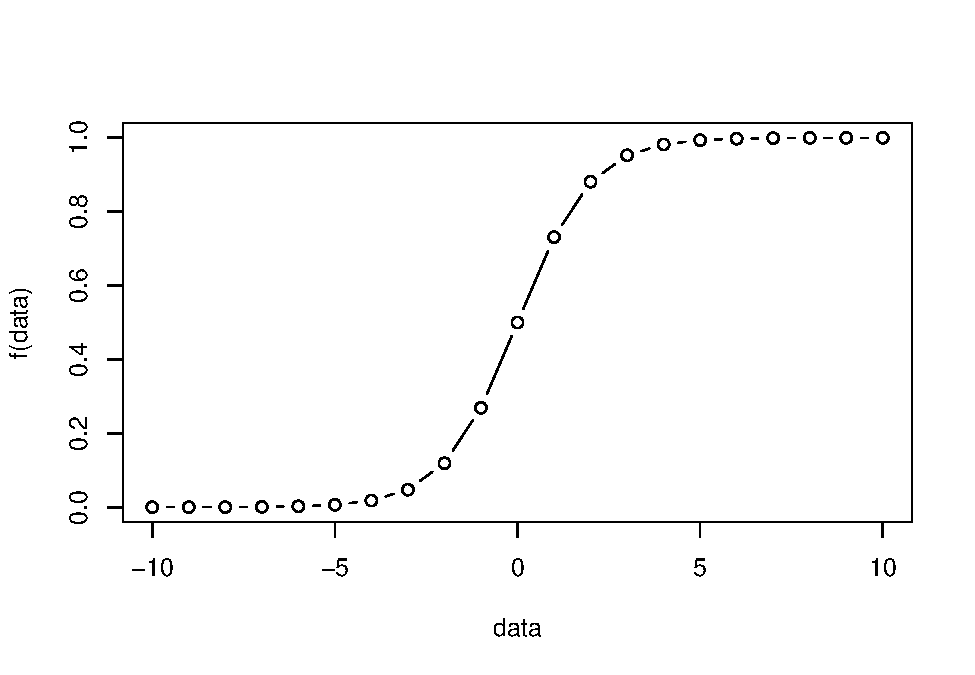
\includegraphics{bookdown-demo_files/figure-latex/unnamed-chunk-1-1.pdf}

We can also write the function into another format as follows:
\[log \frac{p(y=1)}{1-p(y=1)}= \beta_0+\beta_1x_1+...+\beta_nx_n\]
Thus, we know that the regression coeficients of \(\beta_i\) actually change the ``log-odds'' of the event. Of course, note that the magnitude of \(\beta_i\) is dependent upon the units of \(x_i\).

The following is an example testing whether that home teams are more likely to win in NFL games. The results show that the odd of winning is the same for both home and away teams.

\begin{Shaded}
\begin{Highlighting}[]
\NormalTok{mydata =}\StringTok{ }\KeywordTok{read.csv}\NormalTok{(}\KeywordTok{url}\NormalTok{(}\StringTok{'https://raw.githubusercontent.com/nfl-football-ops/Big-Data-Bowl/master/Data/games.csv'}\NormalTok{))}
\NormalTok{mydata}\OperatorTok{$}\NormalTok{result_new<-}\KeywordTok{ifelse}\NormalTok{(mydata}\OperatorTok{$}\NormalTok{HomeScore}\OperatorTok{>}\NormalTok{mydata}\OperatorTok{$}\NormalTok{VisitorScore,}\DecValTok{1}\NormalTok{,}\DecValTok{0}\NormalTok{)}
\KeywordTok{summary}\NormalTok{(mydata}\OperatorTok{$}\NormalTok{result_new)}
\end{Highlighting}
\end{Shaded}

\begin{verbatim}
##    Min. 1st Qu.  Median    Mean 3rd Qu.    Max. 
##  0.0000  0.0000  0.0000  0.4945  1.0000  1.0000
\end{verbatim}

\begin{Shaded}
\begin{Highlighting}[]
\NormalTok{mylogit1 =}\StringTok{ }\KeywordTok{glm}\NormalTok{(result_new}\OperatorTok{~}\DecValTok{1}\NormalTok{, }\DataTypeTok{family=}\NormalTok{binomial, }\DataTypeTok{data=}\NormalTok{mydata)}
\KeywordTok{summary}\NormalTok{(mylogit1)}
\end{Highlighting}
\end{Shaded}

\begin{verbatim}
## 
## Call:
## glm(formula = result_new ~ 1, family = binomial, data = mydata)
## 
## Deviance Residuals: 
##    Min      1Q  Median      3Q     Max  
## -1.168  -1.168  -1.168   1.187   1.187  
## 
## Coefficients:
##             Estimate Std. Error z value Pr(>|z|)
## (Intercept) -0.02198    0.20967  -0.105    0.917
## 
## (Dispersion parameter for binomial family taken to be 1)
## 
##     Null deviance: 126.14  on 90  degrees of freedom
## Residual deviance: 126.14  on 90  degrees of freedom
## AIC: 128.14
## 
## Number of Fisher Scoring iterations: 3
\end{verbatim}

\hypertarget{probit}{%
\section{Probit}\label{probit}}

As noted above, logit \(f(x)=log(\frac{p(y=1)}{1-p(y=1)})\) provides the resulting range of \((0,1)\). Another way to provide the same rage is through the cdf of normal distribution.The following R code is used to illusrate this process.

\begin{Shaded}
\begin{Highlighting}[]
\NormalTok{data2<-}\KeywordTok{seq}\NormalTok{(}\OperatorTok{-}\DecValTok{5}\NormalTok{,}\DecValTok{5}\NormalTok{,}\DecValTok{1}\NormalTok{)}
\KeywordTok{plot}\NormalTok{(data2,}\KeywordTok{pnorm}\NormalTok{(data2),}\DataTypeTok{type =} \StringTok{"b"}\NormalTok{)}
\end{Highlighting}
\end{Shaded}

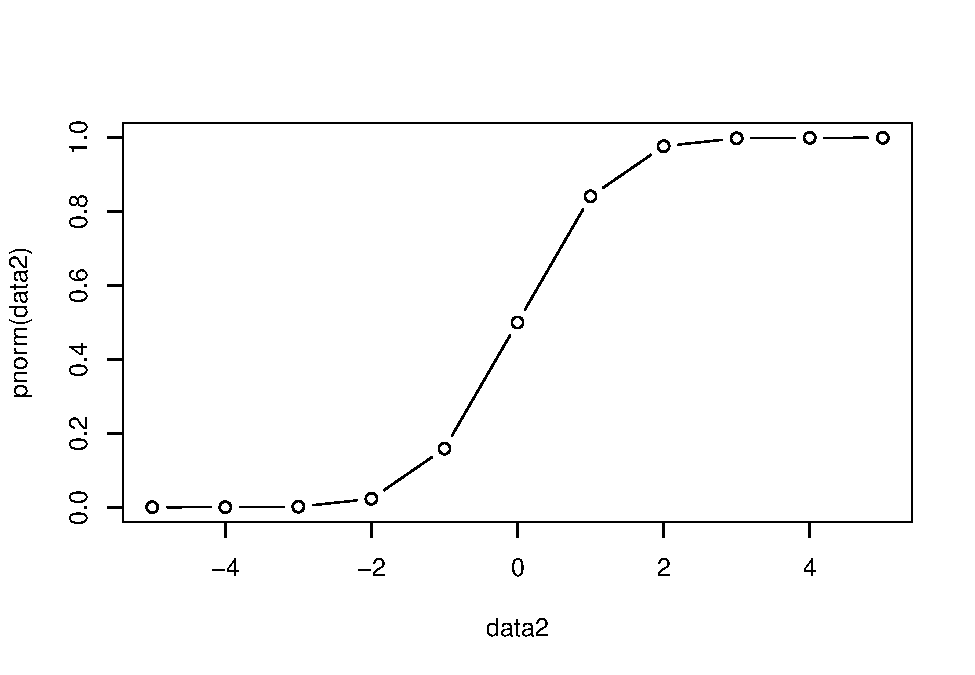
\includegraphics{bookdown-demo_files/figure-latex/unnamed-chunk-3-1.pdf}
Thus, the cdf of normal distribution can be used to indicate the probability of \(p(y=1)\).

\[\Phi(\beta_0+\beta_1x_1+...+\beta_nx_n )= p(y=1)\]

Similar to logit model, we can also write the inverse function of the cdf to get the function that can be from \(-\infty\) to \(+\infty\).

\[\beta_0+\beta_1x_1+...+\beta_nx_n =\Phi^{-1}(p(y=1))\]

Thus, for example, if \(X\beta\) = -2, based on \(\Phi(\beta_0+\beta_1x_1+...+\beta_nx_n )= p(y=1)\) we can get that the \(p(y=1)=0.023\).

In contrast, if \(X\beta\) = 3, the \(p(y=1)=0.999\).

\begin{Shaded}
\begin{Highlighting}[]
\KeywordTok{pnorm}\NormalTok{(}\OperatorTok{-}\DecValTok{2}\NormalTok{)}
\end{Highlighting}
\end{Shaded}

\begin{verbatim}
## [1] 0.02275013
\end{verbatim}

\begin{Shaded}
\begin{Highlighting}[]
\KeywordTok{pnorm}\NormalTok{(}\DecValTok{3}\NormalTok{)}
\end{Highlighting}
\end{Shaded}

\begin{verbatim}
## [1] 0.9986501
\end{verbatim}

Let's assume that there is a latent variable called \(Y^*\) such that

\[Y^*=X\beta+\epsilon, \epsilon \sim N(0,\sigma^2)\]
You could think of \(Y^*\) as a kind of ``proxy'' between \(X\beta+\epsilon\) and the observed \(Y (1 or 0)\). Thus, we can get the following. Note that, it does not have to be zero, and can be any constant.

\[
Y^*=\begin{cases} 0 \;\;\: if \;  y_i^* \leq 0 \\ 1 \;\;\: if \;  y_i^* > 0 \end{cases}
\]

Thus,

\[y_i^* > 0 \Rightarrow \beta^{'}X_i + \epsilon_i >0 \Rightarrow \epsilon_i > -\beta^{'}X_i\]

Thus, we can write it as follows. Note that \(\frac{ \epsilon_i}{\sigma} \sim N(0,1)\)

\[p(y=1|x_i)= p(y_i^* >0|x_i)=p(\epsilon_i > -\beta^{'}X_i)= p(\frac{ \epsilon_i}{\sigma}>\frac{-\beta^{'}X_i}{\sigma})=\Phi(\frac{\beta^{'}X_i}{\sigma}) \]
We thus can get:

\[p(y=0|x_i)=1-\Phi(\frac{\beta^{'}X_i}{\sigma})\]

For \(p(y=1|x_i)=\Phi(\frac{\beta^{'}X_i}{\sigma})\), we can not really estimate both \(\beta\) and \(\sigma\) as they are in a ratio. We can assume \(\sigma =1\), then \(\epsilon \sim N(0,1)\).
We know \(y_i\) and \(x_i\) since we observe them. Thus, we can write it as follows.

\[p(y=1|x_i)=\Phi(\beta^{'}X_i)\]

\hypertarget{normal-distribution}{%
\chapter{Normal distribution}\label{normal-distribution}}

\hypertarget{basics}{%
\section{Basics}\label{basics}}

\(\mu\) and \(\sigma\) determine the center and spread of the distribution.

\begin{figure}
\centering
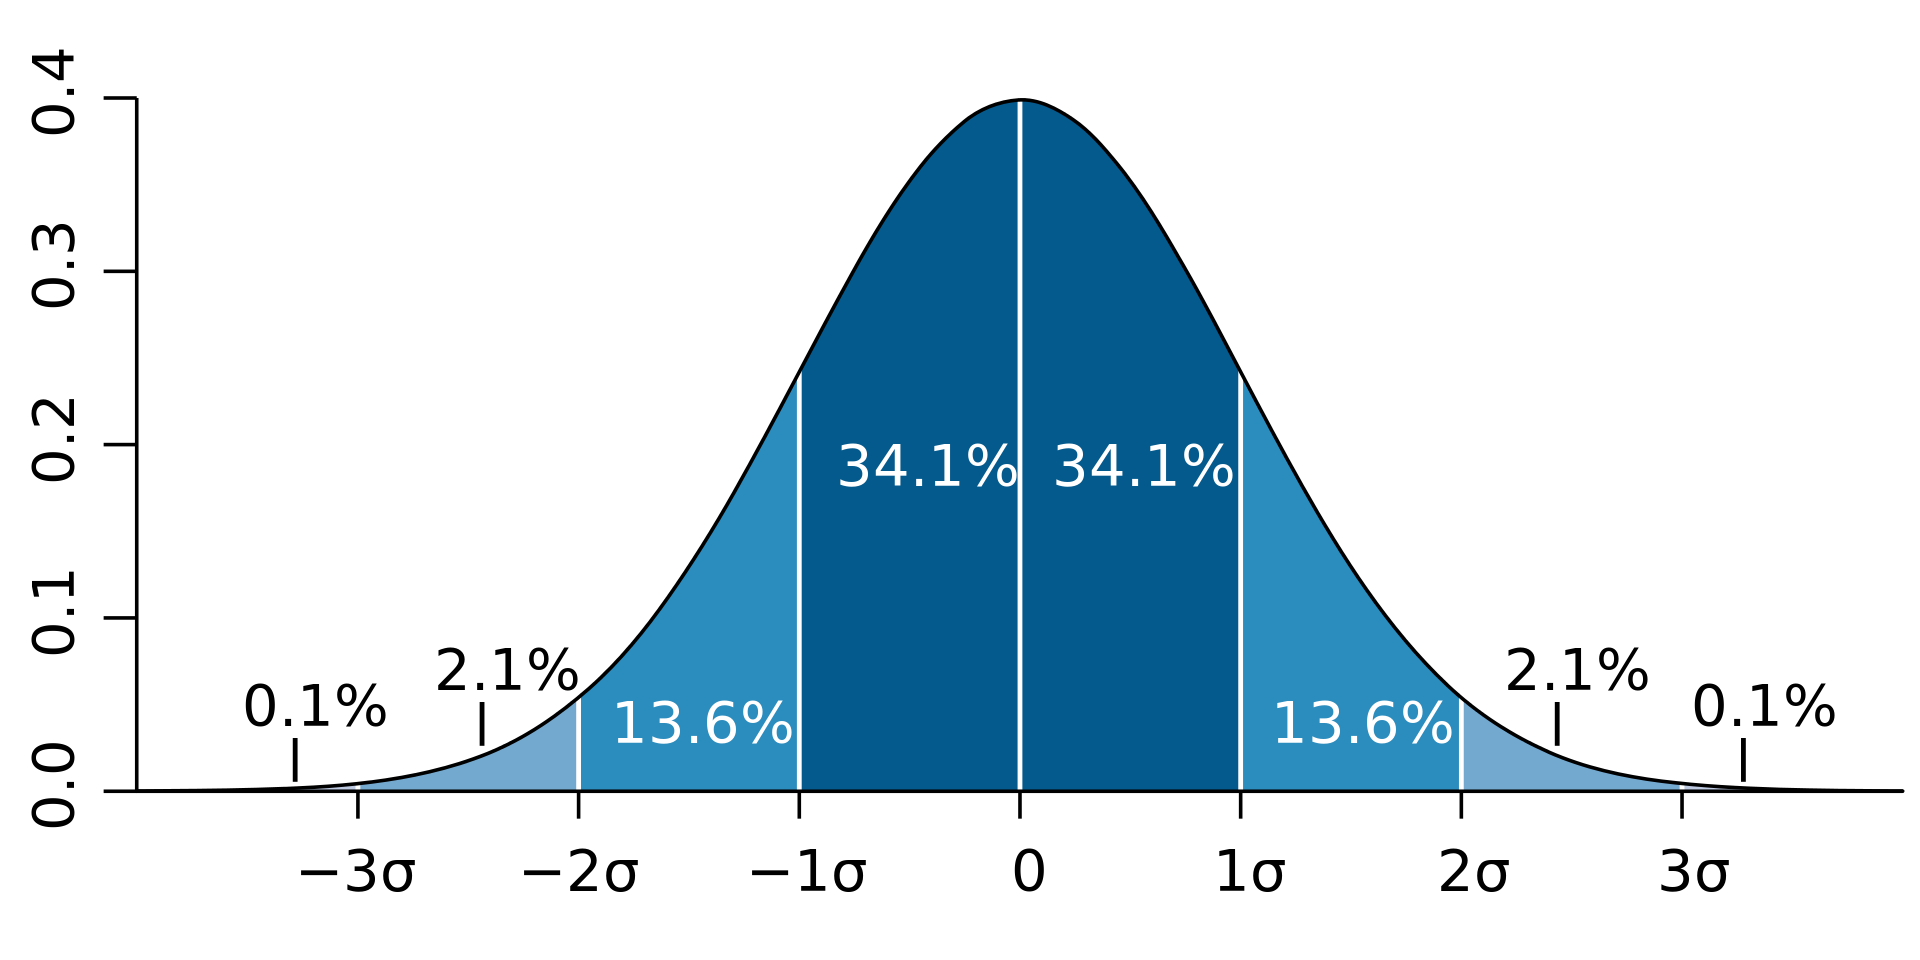
\includegraphics{Standard_deviation_diagram.PNG}
\caption{Normal}
\end{figure}

The empirical rule holds for all normal distributions:

\begin{enumerate}
\def\labelenumi{(\arabic{enumi})}
\item
  68\% of the area under the curve lies between \((\mu-\sigma,\mu+\sigma)\).
\item
  95\% of the area under the curve lies between \((\mu-2\sigma,\mu+2\sigma)\).
\item
  99.7\% of the area under the curve lies between \((\mu-3\sigma,\mu+3\sigma)\).
\end{enumerate}

\hypertarget{confidence-intervals-for-normal-distributions}{%
\section{Confidence intervals for normal distributions}\label{confidence-intervals-for-normal-distributions}}

\[\bar{X} \pm Z \frac{\sigma}{\sqrt{n}}\]
where,

\(\bar{X}\) is the mean

\(Z\) is the Z value (see the table below)

\(\sigma\) is the standard deviation

\(n\) is the number of observations

(We can see the connection between this formula and information shown in the \emph{Basics} section.)

\[\begin{bmatrix}
Confidence \; Levels & Z \\
80  & 1.282 \\
85 & 1.440 \\
90 & 1.645 \\
95 & 1.960 \\
99 & 2.576 \\
99.5 & 2.807 \\
99.9 & 3.291 \end{bmatrix}\]

\hypertarget{percentile}{%
\section{Percentile}\label{percentile}}

A percentile is a measure used in statistics indicating the value below which a given percentage of observations in a group of observations falls.

For example, the 20th percentile is the value (or score) below which 20\% of the observations may be found.

For normal distribution,

-3 \(\sigma\) is the 0.13th percentile (i.e., \(\frac{100-99.7}{2}=0.15\));

-2 \(\sigma\) is the 2.28th percentile ((i.e., \(\frac{100-95}{2}=2.50\)));

-1\(\sigma\) is the 15.87th percentile (i.e., \(\frac{100-68}{2}=16\));

0 \(\sigma\) is 50th percentile.

+2 \(\sigma\) is the 97.72nd percentile (i.e., \(100-\frac{100-95}{2}=100-2.5=97.50\));

+3 \(\sigma\) is the 99.87th percentile (i.e., \(100-\frac{100-99.70}{2}=100-0.15=99.85\)).

This is related to the 68-95-99.7 rule or the three-sigma rule.

(Note that, it is \emph{related}, not \emph{direct} 68-95-99.7 rule, which is about symmetric situations. See the figure above)

\[\begin{bmatrix}
Percentile & Z \\
90  & 1.282 \\
- & 1.440 \\
95 & 1.645 \\
- & 1.960 \\
- & 2.576 \\
- & 2.807 \\
99.9 & 3.000 \end{bmatrix}\]

\hypertarget{intro}{%
\chapter{MLE}\label{intro}}

\hypertarget{basic-idea-of-mle}{%
\section{Basic idea of MLE}\label{basic-idea-of-mle}}

Suppose that we flip a coin, \(y_i=0\) for tails and \(y_i=1\) for heads. If we get \(p\) heads from \(n\) trials, we can get the proportion of heads is \(p/n\), which is the sample mean. If we do not do any further calculation, this is our best guess.

Suppose that the true proablity is \(\rho\), then we can get:

\[
\mathbf{L}(y_i)=\begin{cases} \rho \;\;\:   y_i = 1 \\ 1-\rho \;\;\:  y_i = 0 \end{cases}
\]
Thus, we can also write it as follows.
\[\mathbf{L}(y_i) = \rho^{y_i}(1-\rho)^{1-y_i}\]

Thus, we can get:

\[\prod \mathbf{L}(y_i|\rho)=\rho^{\sum y_i}(1-\rho)^{\sum(1-y_i)}\]
Further, we can get a log-transformed format.

\[log (\prod \mathbf{L}(y_i|\rho))=\sum y_i log \rho + \sum(1-y_i) log(1-\rho)\]

To maximize the log-function above, we can calculate the derivative with respect to \(\rho\).
\[\frac{\partial log (\prod \mathbf{L}(y_i|\rho)) }{\partial \rho}=\sum y_i \frac{1}{\rho}-\sum(1-y_i) \frac{1}{1-\rho}\]
Set the derivative to zero and solve for \(\rho\), we can get

\[\sum y_i \frac{1}{\rho}-\sum(1-y_i) \frac{1}{1-\rho}=0\]
\[\Rightarrow (1-\rho)\sum y_i - \rho \sum(1-y_i) =0\]
\[\Rightarrow \sum y_i-\rho\sum y_i - n\rho +\rho\sum y_i =0\]
\[\Rightarrow \sum y_i - n\rho  =0\]
\[\Rightarrow \rho  = \frac{\sum y_i}{n}=\frac{p}{n}\]
Thus, we can see that the \(\rho\) maximizing the likelihood function is equal to the sample mean.

\hypertarget{coin-flip-example-probit-and-logit}{%
\section{Coin flip example, probit, and logit}\label{coin-flip-example-probit-and-logit}}

In the example above, we are not really trying to estimate a lot of regression coefficients. What we are doing actually is to calculate the sample mean, or intercept in the regresion sense. What does it mean? Let's use some data to explain it.

Suppose that we flip a coin 20 times and observe 8 heads. We can use the R's glm function to esimate the \(\rho\). If the result is consistent with what we did above, we should observe that the \(cdf\) of the esimate of \(\beta_0\) (i.e., intercept) should be equal to \(8/20=0.4\).

\begin{Shaded}
\begin{Highlighting}[]
\NormalTok{coins<-}\KeywordTok{c}\NormalTok{(}\KeywordTok{rep}\NormalTok{(}\DecValTok{1}\NormalTok{,}\DataTypeTok{times=}\DecValTok{8}\NormalTok{),}\KeywordTok{rep}\NormalTok{(}\DecValTok{0}\NormalTok{,}\DataTypeTok{times=}\DecValTok{12}\NormalTok{))}
\KeywordTok{table}\NormalTok{(coins)}
\end{Highlighting}
\end{Shaded}

\begin{verbatim}
## coins
##  0  1 
## 12  8
\end{verbatim}

\begin{Shaded}
\begin{Highlighting}[]
\NormalTok{coins<-}\KeywordTok{as.data.frame}\NormalTok{(coins)}
\end{Highlighting}
\end{Shaded}

\hypertarget{probit-1}{%
\subsection{Probit}\label{probit-1}}

\begin{Shaded}
\begin{Highlighting}[]
\NormalTok{probitresults <-}\StringTok{ }\KeywordTok{glm}\NormalTok{(coins }\OperatorTok{~}\StringTok{ }\DecValTok{1}\NormalTok{, }\DataTypeTok{family =} \KeywordTok{binomial}\NormalTok{(}\DataTypeTok{link =} \StringTok{"probit"}\NormalTok{), }\DataTypeTok{data =}\NormalTok{ coins)}
\NormalTok{probitresults}
\end{Highlighting}
\end{Shaded}

\begin{verbatim}
## 
## Call:  glm(formula = coins ~ 1, family = binomial(link = "probit"), 
##     data = coins)
## 
## Coefficients:
## (Intercept)  
##     -0.2533  
## 
## Degrees of Freedom: 19 Total (i.e. Null);  19 Residual
## Null Deviance:       26.92 
## Residual Deviance: 26.92     AIC: 28.92
\end{verbatim}

\begin{Shaded}
\begin{Highlighting}[]
\KeywordTok{pnorm}\NormalTok{(probitresults}\OperatorTok{$}\NormalTok{coefficients)}
\end{Highlighting}
\end{Shaded}

\begin{verbatim}
## (Intercept) 
##         0.4
\end{verbatim}

As we can see the intercept is \(-0.2533\), and thus \(\Phi(-0.2533471)=0.4\)

\hypertarget{logit-1}{%
\subsection{Logit}\label{logit-1}}

We can also use logit link to calculate the intercept as well. Recall that

\[p(y=1)=\frac{1}{1+e^{-(\beta_0+\beta_1x_1+...+\beta_nx_n)}}=\frac{e^{\beta_0+\beta_1x_1+...+\beta_nx_n}}{1+e^{\beta_0+\beta_1x_1+...+\beta_nx_n}}\]
Thus,

\[p(y=1)=\frac{e^{\beta_0}}{1+e^{\beta_0}}\]

\begin{Shaded}
\begin{Highlighting}[]
\NormalTok{logitresults <-}\StringTok{ }\KeywordTok{glm}\NormalTok{(coins }\OperatorTok{~}\StringTok{ }\DecValTok{1}\NormalTok{, }\DataTypeTok{family =} \KeywordTok{binomial}\NormalTok{(}\DataTypeTok{link =} \StringTok{"logit"}\NormalTok{), }\DataTypeTok{data =}\NormalTok{ coins)}
\NormalTok{logitresults}\OperatorTok{$}\NormalTok{coefficients}
\end{Highlighting}
\end{Shaded}

\begin{verbatim}
## (Intercept) 
##  -0.4054651
\end{verbatim}

\begin{Shaded}
\begin{Highlighting}[]
\KeywordTok{exp}\NormalTok{(logitresults}\OperatorTok{$}\NormalTok{coefficients)}\OperatorTok{/}\NormalTok{(}\DecValTok{1}\OperatorTok{+}\KeywordTok{exp}\NormalTok{(logitresults}\OperatorTok{$}\NormalTok{coefficients))}
\end{Highlighting}
\end{Shaded}

\begin{verbatim}
## (Intercept) 
##         0.4
\end{verbatim}

Note that, the defaul link for the binomial in the glm function in logit.

\hypertarget{further-on-logit}{%
\section{Further on logit}\label{further-on-logit}}

The probablity of \(y=1\) is as follows:

\[p=p(y=1)=\frac{1}{1+e^{-(\beta_0+\beta_1x_1+...+\beta_nx_n)}}=\frac{e^{\beta_0+\beta_1x_1+...+\beta_nx_n}}{1+e^{\beta_0+\beta_1x_1+...+\beta_nx_n}}\]

Thus, the likelihood function is as follows:

\[L=\prod p^{y_i}(1-p)^{1-y_i}=\prod (\frac{1}{1+e^{-(\beta_0+\beta_1x_1+...+\beta_nx_n)}})^{y_i}(\frac{1}{1+e^{\beta_0+\beta_1x_1+...+\beta_nx_n}})^{1-y_i}\]

\[=\prod (1+e^{-(\beta_0+\beta_1x_1+...+\beta_nx_n)})^{-y_i}(1+e^{\beta_0+\beta_1x_1+...+\beta_nx_n})^{-(1-y_i)}\]

Thus, the log-likelihood is as follows:
\[logL=\sum (-y_i \cdot log(1+e^{-(\beta_0+\beta_1x_1+...+\beta_nx_n)})-(1-y_i)\cdot log(1+e^{\beta_0+\beta_1x_1+...+\beta_nx_n}))\]

Typically, optimisers minimize a function, so we use negative log-likelihood as minimising that is equivalent to maximising the log-likelihood or the likelihood itself.

\begin{Shaded}
\begin{Highlighting}[]
\CommentTok{#Source of R code: https://www.r-bloggers.com/logistic-regression/}

\NormalTok{mle.logreg =}\StringTok{ }\ControlFlowTok{function}\NormalTok{(fmla, data)}
\NormalTok{\{}
  \CommentTok{# Define the negative log likelihood function}
\NormalTok{  logl <-}\StringTok{ }\ControlFlowTok{function}\NormalTok{(theta,x,y)\{}
\NormalTok{    y <-}\StringTok{ }\NormalTok{y}
\NormalTok{    x <-}\StringTok{ }\KeywordTok{as.matrix}\NormalTok{(x)}
\NormalTok{    beta <-}\StringTok{ }\NormalTok{theta[}\DecValTok{1}\OperatorTok{:}\KeywordTok{ncol}\NormalTok{(x)]}
    
    \CommentTok{# Use the log-likelihood of the Bernouilli distribution, where p is}
    \CommentTok{# defined as the logistic transformation of a linear combination}
    \CommentTok{# of predictors, according to logit(p)=(x%*%beta)}
\NormalTok{    loglik <-}\StringTok{ }\KeywordTok{sum}\NormalTok{(}\OperatorTok{-}\NormalTok{y}\OperatorTok{*}\KeywordTok{log}\NormalTok{(}\DecValTok{1} \OperatorTok{+}\StringTok{ }\KeywordTok{exp}\NormalTok{(}\OperatorTok{-}\NormalTok{(x}\OperatorTok\NormalTok{beta))) }\OperatorTok{-}\StringTok{ }\NormalTok{(}\DecValTok{1}\OperatorTok{-}\NormalTok{y)}\OperatorTok{*}\KeywordTok{log}\NormalTok{(}\DecValTok{1} \OperatorTok{+}\StringTok{ }\KeywordTok{exp}\NormalTok{(x}\OperatorTok\NormalTok{beta)))}
    \KeywordTok{return}\NormalTok{(}\OperatorTok{-}\NormalTok{loglik)}
\NormalTok{  \}}
  
  \CommentTok{# Prepare the data}
\NormalTok{  outcome =}\StringTok{ }\KeywordTok{rownames}\NormalTok{(}\KeywordTok{attr}\NormalTok{(}\KeywordTok{terms}\NormalTok{(fmla),}\StringTok{"factors"}\NormalTok{))[}\DecValTok{1}\NormalTok{]}
\NormalTok{  dfrTmp =}\StringTok{ }\KeywordTok{model.frame}\NormalTok{(data)}
\NormalTok{  x =}\StringTok{ }\KeywordTok{as.matrix}\NormalTok{(}\KeywordTok{model.matrix}\NormalTok{(fmla, }\DataTypeTok{data=}\NormalTok{dfrTmp))}
\NormalTok{  y =}\StringTok{ }\KeywordTok{as.numeric}\NormalTok{(}\KeywordTok{as.matrix}\NormalTok{(data[,}\KeywordTok{match}\NormalTok{(outcome,}\KeywordTok{colnames}\NormalTok{(data))]))}
  
  \CommentTok{# Define initial values for the parameters}
\NormalTok{  theta.start =}\StringTok{ }\KeywordTok{rep}\NormalTok{(}\DecValTok{0}\NormalTok{,(}\KeywordTok{dim}\NormalTok{(x)[}\DecValTok{2}\NormalTok{]))}
  \KeywordTok{names}\NormalTok{(theta.start) =}\StringTok{ }\KeywordTok{colnames}\NormalTok{(x)}
  
  \CommentTok{# Calculate the maximum likelihood}
\NormalTok{  mle =}\StringTok{ }\KeywordTok{optim}\NormalTok{(theta.start,logl,}\DataTypeTok{x=}\NormalTok{x,}\DataTypeTok{y=}\NormalTok{y, }\DataTypeTok{method =} \StringTok{'BFGS'}\NormalTok{, }\DataTypeTok{hessian=}\NormalTok{T)}
\NormalTok{  out =}\StringTok{ }\KeywordTok{list}\NormalTok{(}\DataTypeTok{beta=}\NormalTok{mle}\OperatorTok{$}\NormalTok{par,}\DataTypeTok{vcov=}\KeywordTok{solve}\NormalTok{(mle}\OperatorTok{$}\NormalTok{hessian),}\DataTypeTok{ll=}\DecValTok{2}\OperatorTok{*}\NormalTok{mle}\OperatorTok{$}\NormalTok{value)}
\NormalTok{\}}
\end{Highlighting}
\end{Shaded}

\begin{Shaded}
\begin{Highlighting}[]
\NormalTok{mydata =}\StringTok{ }\KeywordTok{read.csv}\NormalTok{(}\KeywordTok{url}\NormalTok{(}\StringTok{'https://stats.idre.ucla.edu/stat/data/binary.csv'}\NormalTok{))}
\NormalTok{mylogit1 =}\StringTok{ }\KeywordTok{glm}\NormalTok{(admit}\OperatorTok{~}\NormalTok{gre}\OperatorTok{+}\NormalTok{gpa}\OperatorTok{+}\KeywordTok{as.factor}\NormalTok{(rank), }\DataTypeTok{family=}\NormalTok{binomial, }\DataTypeTok{data=}\NormalTok{mydata)}

\NormalTok{mydata}\OperatorTok{$}\NormalTok{rank =}\StringTok{ }\KeywordTok{factor}\NormalTok{(mydata}\OperatorTok{$}\NormalTok{rank) }\CommentTok{#Treat rank as a categorical variable}
\NormalTok{fmla =}\StringTok{ }\KeywordTok{as.formula}\NormalTok{(}\StringTok{"admit~gre+gpa+rank"}\NormalTok{) }\CommentTok{#Create model formula}
\NormalTok{mylogit2 =}\StringTok{ }\KeywordTok{mle.logreg}\NormalTok{(fmla, mydata) }\CommentTok{#Estimate coefficients}


 \KeywordTok{print}\NormalTok{(}\KeywordTok{cbind}\NormalTok{(}\KeywordTok{coef}\NormalTok{(mylogit1), mylogit2}\OperatorTok{$}\NormalTok{beta))}
\end{Highlighting}
\end{Shaded}

\begin{verbatim}
##                          [,1]         [,2]
## (Intercept)      -3.989979073 -3.772676422
## gre               0.002264426  0.001375522
## gpa               0.804037549  0.898201239
## as.factor(rank)2 -0.675442928 -0.675543009
## as.factor(rank)3 -1.340203916 -1.356554831
## as.factor(rank)4 -1.551463677 -1.563396035
\end{verbatim}

\hypertarget{references}{%
\section{References}\label{references}}

\url{http://www.columbia.edu/~so33/SusDev/Lecture_9.pdf}

\hypertarget{score-gradient-and-jacobian}{%
\chapter{Score, Gradient and Jacobian}\label{score-gradient-and-jacobian}}

\hypertarget{score}{%
\section{Score}\label{score}}

The score is the gradient (the vector of partial derivatives) of \(log L(\theta)\), with respect to an m-dimensional parameter vector \(\theta\).

\[S(\theta) = \frac{\partial\ell}{\partial \theta}\]
Typically, they use \(\nabla\) to denote the partical derivative.

\[\nabla \ell\]

Such differentiation will generate a \(m \times 1\) row vector, which indicates the sensitivity of the likelihood.

Quote from Steffen Lauritzen's slides: ``Generally the solution to this equation must be calculated by iterative methods. One of the most common methods is the Newton--Raphson
method and this is based on successive approximations to the solution, using Taylor's theorem to approximate the equation.''

For instance, using logit link, we can get the first derivative of log likelihood logistic regression as follows. We can not really find \(\beta\) easily to make the equation to be 0.

\[\begin{aligned}
\frac{\partial \ell} {\partial \beta} 
&= \sum_{i=1}^{n}x_i^T[y_i-\frac{e^{\beta^Tx_i}}{1+e^{\beta^Tx_i}}] \\
&=\sum_{i=1}^{n} x_i^T[y_i-\hat{y_i}]
\end{aligned}\]

\hypertarget{fisher-scoring}{%
\section{Fisher scoring}\label{fisher-scoring}}

{[}I will come back to this later.{]}

\url{https://www2.stat.duke.edu/courses/Fall00/sta216/handouts/diagnostics.pdf}

\url{https://stats.stackexchange.com/questions/176351/implement-fisher-scoring-for-linear-regression}

\hypertarget{gradient-and-jacobian}{%
\section{Gradient and Jacobian}\label{gradient-and-jacobian}}

\textbf{Remarks}: This part discusses gradient in a more general sense.

When \(f(x)\) is only in a single dimension space:

\(\mathbb{R}^n \rightarrow \mathbb{R}\)

\[\nabla f(x)=[\frac{\partial f}{\partial x_1},\frac{\partial f}{\partial x_2},...,\frac{\partial f}{\partial x_n}]\]
When \(f(x)\) is only in a m-dimension space (i.e., Jacobian):
\(\mathbb{R}^n \rightarrow \mathbb{R^m}\)

\[Jac(f)=\begin{bmatrix}
\frac{\partial f_1}{\partial x_1} & \frac{\partial f_1}{\partial x_2} & \frac{\partial f_1}{\partial x_3} & ... & \frac{\partial f_1}{\partial x_n}\\
\frac{\partial f_2}{\partial x_1} & \frac{\partial f_2}{\partial x_2} & \frac{\partial f_2}{\partial x_3} & ... & \frac{\partial f_2}{\partial x_n} \\
...\\
\frac{\partial f_m}{\partial x_1} & \frac{\partial f_m}{\partial x_2} & \frac{\partial f_n}{\partial x_3} & ... & \frac{\partial f_m}{\partial x_n}
\end{bmatrix}\]

For instance,

\(\mathbb{R}^n \rightarrow \mathbb{R}\):

\[f(x,y)=x^2+2y\]
\[\nabla f(x,y)=[\frac{\partial f}{\partial x},\frac{\partial f}{\partial y}]=[2x,2]\]
\(\mathbb{R}^n \rightarrow \mathbb{R^m}\)

\[f(x,y)=(x^2+2y,x^3)\]
\[Jac(f)=\begin{bmatrix}
2x & 2\\
2x^2 & 0 
\end{bmatrix}\]

\hypertarget{hessian-and-fisher-information}{%
\section{Hessian and Fisher Information}\label{hessian-and-fisher-information}}

Hessian matrix or Hessian is a square matrix of second-order partial derivatives of a scalar-valued function, or scalar field.

\(\mathbb{R}^n \rightarrow \mathbb{R}\)

\[Hessian=\nabla ^2(f) =\begin{bmatrix}
\frac{\partial^2 f}{\partial x_1^2} & \frac{\partial^2 f}{\partial x_1 \partial x_2} & \frac{\partial^2 f}{\partial x_1 \partial x_3} & ... & \frac{\partial^2 f}{\partial x_1 \partial x_n}\\
\frac{\partial^2 f}{\partial x_2 \partial x_1} & \frac{\partial^2 f}{\partial x_2^2} & \frac{\partial^2 f}{\partial x_2 \partial x_3} & ... & \frac{\partial^2 f}{\partial x_2 \partial x_n} \\
\frac{\partial^2 f}{\partial x_3 \partial x_1} & \frac{\partial^2 f}{\partial x_3 \partial x_2} & \frac{\partial^2 f}{\partial x_3^2} & ... & \frac{\partial^2 f}{\partial x_3 \partial x_n} \\
...\\
\frac{\partial^2 f}{\partial x_n \partial x_1} & \frac{\partial^2 f}{\partial x_n \partial x_2} & \frac{\partial^2 f}{\partial x_n \partial x_3} & ... & \frac{\partial^2 f}{\partial x_n^2}
\end{bmatrix}\]

As a special case, in the context of logit:

Suppose that the log likelihood function is \(\ell (\theta)\). \(\theta\) is a \(m\) demension vector.

\[ \theta = \begin{bmatrix}\theta_1 \\
\theta_2 \\
\theta_3 \\
\theta_4 \\
...\\
\theta_m \\
\end{bmatrix}\]

\[Hessian=\nabla ^2(\ell) =\begin{bmatrix}
\frac{\partial^2 \ell}{\partial \theta_1^2} & \frac{\partial^2 \ell}{\partial \theta_1 \partial \theta_2} & \frac{\partial^2 \ell}{\partial \theta_1 \partial \theta_3} & ... & \frac{\partial^2 \ell}{\partial \theta_1 \partial \theta_m}\\
\frac{\partial^2 \ell}{\partial \theta_2 \partial \theta_1} & \frac{\partial^2 \ell}{\partial \theta_2^2 } & \frac{\partial^2 \ell}{\partial \theta_1 \partial \theta_3} & ... & \frac{\partial^2 \ell}{\partial \theta_1 \partial \theta_m} \\
\frac{\partial^2 \ell}{\partial \theta_3 \partial \theta_1} & \frac{\partial^2 \ell}{\partial \theta_3 \theta_2 } & \frac{\partial^2 \ell}{\partial \theta_3^2} & ... & \frac{\partial^2 \ell}{\partial \theta_3 \partial \theta_m} \\
...\\
\frac{\partial^2 \ell}{\partial \theta_m \partial \theta_1} & \frac{\partial^2 \ell}{\partial \theta_m \theta_2 } & \frac{\partial^2 \ell}{\partial \theta_m \partial \theta_3} & ... & \frac{\partial^2 \ell}{\partial \theta_m \partial \theta_m} 
\end{bmatrix}\]

``In statistics, the observed information, or observed Fisher information, is the negative of the second derivative (the Hessian matrix) of the''log-likelihood" (the logarithm of the likelihood function). It is a sample-based version of the Fisher information." (Direct quote from Wikipedia.)

Thus, the observed information matrix:

\[-Hessian=-\nabla ^2(\ell) \]

Expected (Fisher) information matrix:

\[E[-\nabla ^2(\ell)] \]

\hypertarget{canonical-link-function}{%
\chapter{Canonical link function}\label{canonical-link-function}}

Inspired by a Stack Exchange post, I created the following figure:

\[ \frac{Paramter}{\theta} \longrightarrow \gamma^{'}(\theta) = \mu \longrightarrow \frac{Mean}{\mu} \longrightarrow g(\mu) = \eta \longrightarrow \frac{ Linear predictor}{\eta} \]

For the case of \(n\) time Bernoulli (i.e., Binomial), its canonical link function is logit. Specifically,

\[ \frac{Paramter}{\theta=\beta^Tx_i}  \longrightarrow \gamma^{'}(\theta)= \frac{e^{\beta^Tx_i}}{1+e^{\beta^Tx_i}}\longrightarrow \frac{Mean}{\mu=\frac{e^{\beta^Tx_i}}{1+e^{\beta^Tx_i}}}\longrightarrow g(\mu) = log \frac{\frac{e^{\beta^Tx_i}}{1+e^{\beta^Tx_i}}}{1-\frac{e^{\beta^Tx_i}}{1+e^{\beta^Tx_i}}}\longrightarrow \frac{ Linear predictor}{\eta = \beta^Tx_i}\]
Thus, we can see that,

\[\theta \equiv \eta \]
The link function \(g(\mu)\) relates the linear predictor \(\eta = \beta^Tx_i\) to the mean \(\mu\).

\textbf{Remarks}:

\begin{enumerate}
\def\labelenumi{(\arabic{enumi})}
\item
  Parameter is \(\theta = \beta ^T x_i\) (Not \(\mu\)!).
\item
  \(\mu=p(y=1)=\frac{e^{\beta^Tx_i}}{1+e^{\beta^Tx_i}}\) (Not logit!).
\item
  Link function (i.e., \(g(\mu)\)) = logit = logarithm of odds = log \(\frac{Event - Happened }{Event - Not - Happened}\).
\item
  \(g(\mu) = log \frac{\mu}{1-\mu}=\beta^T x_i\). Thus, link function = linear predictor = log odds!
\item
  Quote from the Stack Exchange post ``Newton Method and Fisher scoring for finding the ML estimator coincide, these links simplify the derivation of the MLE.''
\end{enumerate}

(Recall, we know that \(\mu\) or \(p(y=1)\) is the mean function. Recall that, \(n\) trails of coin flips, and get \(p\) heads. Thus \(\mu = \frac{p}{n}\).)

\hypertarget{ordinary-least-squares-ols}{%
\chapter{Ordinary Least Squares (OLS)}\label{ordinary-least-squares-ols}}

Suppose we have \(n\) observation, and \(m\) variables.

\[\begin{bmatrix}
x_{11} & x_{12} & x_{13} & ... & x_{1m}\\
x_{21} & x_{22} & x_{23} & ... & x_{2m} \\
...\\
x_{n1} & x_{n2} & x_{n3} & ... & x_{nm}
\end{bmatrix}\]

Thus, we can write it as the following \(n\) equations.

\[y_1=\beta_0+\beta_1 x_{11}+\beta_2 x_{12}+...+ \beta_m x_{1m}\]
\[y_2=\beta_0+\beta_1 x_{21}+\beta_2 x_{22}+...+ \beta_m x_{2m}\]
\[y_3=\beta_0+\beta_1 x_{31}+\beta_2 x_{32}+...+ \beta_m x_{3m}\]
\[...\]

\[y_n=\beta_0+\beta_1 x_{n1}+\beta_2 x_{n2}+...+ \beta_m x_{nm}\]

We can combine all the \(n\) equations as the following one:

\[y_i=\beta_0+\beta_1 x_{i1}+\beta_2 x_{i2}+...+ \beta_m x_{im}  (i \in [1,n])\]

We can further rewrite it as a matrix format as follows.

\[y= X \beta\]
Where,

\[y = \begin{bmatrix}y_1 \\
y_2 \\
y_3 \\
y_4 \\
...\\
y_n \\
\end{bmatrix}\]

\[X=\begin{bmatrix}
1 & x_{11} & x_{12} & x_{13} & ... & x_{1m}\\
1 & x_{21} & x_{22} & x_{23} & ... & x_{2m} \\
...\\
1 & x_{n1} & x_{n2} & x_{n3} & ... & x_{nm}
\end{bmatrix}\]

\[\beta = \begin{bmatrix}\beta_0 \\
\beta_1 \\
\beta_2 \\
\beta_3 \\
...\\
\beta_m \\
\end{bmatrix}\]

Since later we need the inverse of \(X\), we need to make it into a square matrix.

\[X^Ty=X^TX \hat{\beta} \Rightarrow \hat{\beta} = (X^TX)^{-1} X^Ty\]

We can use R to implement this calculation. As we can see, there is no need to do any iterations at all, but rather just pure matrix calculation.

\begin{Shaded}
\begin{Highlighting}[]
\NormalTok{X<-}\KeywordTok{matrix}\NormalTok{(}\KeywordTok{rnorm}\NormalTok{(}\DecValTok{1000}\NormalTok{),}\DataTypeTok{ncol=}\DecValTok{2}\NormalTok{) }\CommentTok{# we define a 2 column matrix, with 500 rows}
\NormalTok{X<-}\KeywordTok{cbind}\NormalTok{(}\DecValTok{1}\NormalTok{,X) }\CommentTok{# add a 1 constant}
\NormalTok{beta_true<-}\KeywordTok{c}\NormalTok{(}\DecValTok{2}\NormalTok{,}\DecValTok{1}\NormalTok{,}\DecValTok{2}\NormalTok{) }\CommentTok{# True regression coefficients}
\NormalTok{beta_true<-}\KeywordTok{as.matrix}\NormalTok{(beta_true)}
\NormalTok{y=X}\OperatorTok\NormalTok{beta_true}\OperatorTok{+}\KeywordTok{rnorm}\NormalTok{(}\DecValTok{500}\NormalTok{)}

\NormalTok{transposed_X<-}\KeywordTok{t}\NormalTok{(X)}
\NormalTok{beta_hat<-}\KeywordTok{solve}\NormalTok{(transposed_X}\OperatorTok\NormalTok{X)}\OperatorTok\NormalTok{transposed_X}\OperatorTok\NormalTok{y}
\NormalTok{beta_hat}
\end{Highlighting}
\end{Shaded}

\begin{verbatim}
##          [,1]
## [1,] 1.940647
## [2,] 1.057231
## [3,] 1.990939
\end{verbatim}

\textbf{Side Notes}
The function of as.matrix will automatically make c(2,1,2) become the dimension of \(3 \times 1\), you do not need to transpose the \(\beta\).

\hypertarget{taylor-series}{%
\section{Taylor series}\label{taylor-series}}

\[\begin{aligned}
f(x)|_{a} &=f(a)+\frac{f^{'}(a)}{1!}(x-a)+\frac{f^{'}(a)}{2!}(x-a)^2+\frac{f^{''}(a)}{3!}(x-a)^{3}+...\\&=\sum_{n=0}^{\infty} \frac{f^{n}(a)}{n!}(x-a)^n 
\end{aligned}\]

For example:

\[\begin{aligned} 
e^x |_{a=0} &= e^a+ \frac{e^a}{1!}(x-a)+\frac{e^a}{2!}(x-a)^2+...+\frac{e^a}{n!}(x-a)^n \\ 
&=  1+ \frac{1}{1!}x+\frac{1}{2!}x^2+...+\frac{1}{n!}x^n
\end{aligned}\]

if \(x=2\)

\(e^2 = 7.389056\)

\(e^2 \approx 1+\frac{1}{1!}x =1+\frac{1}{1!}2=3\)

\(e^2 \approx 1+\frac{1}{1!}x+\frac{1}{2!}x^2 =1+\frac{1}{1!}2 + \frac{1}{2!}2 =5\)
\ldots{}

\(e^2 \approx 1+\frac{1}{1!}x+\frac{1}{2!}x^2 +\frac{1}{3!}x^2+\frac{1}{4!}x^2+\frac{1}{5!}x^2=7.2666...\)

\hypertarget{references-1}{%
\section{References}\label{references-1}}

\begin{enumerate}
\def\labelenumi{\arabic{enumi}.}
\tightlist
\item
  Steffen Lauritzen's slides:
\end{enumerate}

\url{http://www.stats.ox.ac.uk/~steffen/teaching/bs2HT9/scoring.pdf}

\begin{enumerate}
\def\labelenumi{\arabic{enumi}.}
\setcounter{enumi}{1}
\tightlist
\item
  The Stack Exchange post:
\end{enumerate}

\url{https://stats.stackexchange.com/questions/40876/what-is-the-difference-between-a-link-function-and-a-canonical-link-function}

\begin{enumerate}
\def\labelenumi{\arabic{enumi}.}
\setcounter{enumi}{2}
\tightlist
\item
  Wilipedia for OLS
\end{enumerate}

\url{https://en.wikipedia.org/wiki/Ordinary_least_squares}

\begin{enumerate}
\def\labelenumi{\arabic{enumi}.}
\setcounter{enumi}{3}
\tightlist
\item
  Gradient and Jacobian
\end{enumerate}

\url{https://math.stackexchange.com/questions/1519367/difference-between-gradient-and-jacobian}

\url{https://www.youtube.com/watch?v=3xVMVT-2_t4}

\url{https://math.stackexchange.com/questions/661195/what-is-the-difference-between-the-gradient-and-the-directional-derivative}

\begin{enumerate}
\def\labelenumi{\arabic{enumi}.}
\setcounter{enumi}{4}
\tightlist
\item
  Hessian
\end{enumerate}

\url{https://en.wikipedia.org/wiki/Hessian_matrix}

\begin{enumerate}
\def\labelenumi{\arabic{enumi}.}
\setcounter{enumi}{5}
\tightlist
\item
  Observed information
\end{enumerate}

\url{https://en.wikipedia.org/wiki/Observed_information}

\begin{enumerate}
\def\labelenumi{\arabic{enumi}.}
\setcounter{enumi}{6}
\tightlist
\item
  Fisher information
\end{enumerate}

\url{https://people.missouristate.edu/songfengzheng/Teaching/MTH541/Lecture\%20notes/Fisher_info.pdf}

\begin{enumerate}
\def\labelenumi{\arabic{enumi}.}
\setcounter{enumi}{7}
\tightlist
\item
  Link function
\end{enumerate}

\url{https://en.wikipedia.org/wiki/Generalized_linear_model\#Link_function}

\url{https://stats.stackexchange.com/questions/40876/what-is-the-difference-between-a-link-function-and-a-canonical-link-function}

\hypertarget{cholesky-decomposition}{%
\chapter{Cholesky decomposition}\label{cholesky-decomposition}}

\hypertarget{example-1}{%
\section{Example 1}\label{example-1}}

Use Cholesky decomposition to generate 1,000 trivariate normal deviates \(X_1, ..., x_{1000}\) with mean \(\mu\) = (−2, 4, 3) and covariance matrix

\[X=\begin{bmatrix}
2 & -1 & 0.5 \\
-1 & 4 & 1 \\
0.5 & 1 & 5 
\end{bmatrix}\]

\begin{Shaded}
\begin{Highlighting}[]
\NormalTok{Nsim =}\StringTok{ }\DecValTok{10}           
\NormalTok{means =}\StringTok{ }\KeywordTok{c}\NormalTok{(}\OperatorTok{-}\DecValTok{2}\NormalTok{,}\DecValTok{4}\NormalTok{,}\DecValTok{3}\NormalTok{)              }
\NormalTok{N_columns =}\StringTok{ }\DecValTok{3}               

\CommentTok{# Generating random standard normal distribution numbers }
\NormalTok{Generated_numbers =}\StringTok{ }\KeywordTok{matrix}\NormalTok{(}\KeywordTok{rnorm}\NormalTok{(N_columns }\OperatorTok{*}\StringTok{ }\NormalTok{Nsim), }\DataTypeTok{nrow =}\NormalTok{ N_columns) }

\CommentTok{# The provided covariance matrix}
\NormalTok{cov_matrix =}\StringTok{ }\KeywordTok{rbind}\NormalTok{(}\KeywordTok{c}\NormalTok{(}\DecValTok{2}\NormalTok{, }\DecValTok{-1}\NormalTok{, }\FloatTok{0.5}\NormalTok{), }\KeywordTok{c}\NormalTok{(}\OperatorTok{-}\DecValTok{1}\NormalTok{, }\DecValTok{4}\NormalTok{, }\DecValTok{1}\NormalTok{), }\KeywordTok{c}\NormalTok{(}\FloatTok{0.5}\NormalTok{, }\DecValTok{1}\NormalTok{, }\DecValTok{5}\NormalTok{))}

\CommentTok{# Cholesky decomposition }
\NormalTok{Cholesky_decom_results =}\StringTok{ }\KeywordTok{chol}\NormalTok{(cov_matrix)    }

\CommentTok{# Data is transformed using the Cholesky decomposition }
\NormalTok{adjusted_data =}\StringTok{ }\KeywordTok{t}\NormalTok{(Generated_numbers) }\OperatorTok\StringTok{ }\NormalTok{Cholesky_decom_results       }

\NormalTok{Final_data =}\StringTok{ }\KeywordTok{t}\NormalTok{(}\KeywordTok{t}\NormalTok{(adjusted_data) }\OperatorTok{+}\StringTok{ }\NormalTok{means)}



\CommentTok{# calculating column means}
\KeywordTok{colMeans}\NormalTok{(Final_data)}
\end{Highlighting}
\end{Shaded}

\begin{verbatim}
## [1] -1.318190  3.435225  3.106621
\end{verbatim}

\begin{Shaded}
\begin{Highlighting}[]
\CommentTok{# calculating column variances}
\KeywordTok{apply}\NormalTok{(Final_data,}\DecValTok{2}\NormalTok{,var)}
\end{Highlighting}
\end{Shaded}

\begin{verbatim}
## [1] 1.483805 5.337909 3.442617
\end{verbatim}

\begin{Shaded}
\begin{Highlighting}[]
\CommentTok{# calculating covariance matrix}
\KeywordTok{cov}\NormalTok{(Final_data)}
\end{Highlighting}
\end{Shaded}

\begin{verbatim}
##            [,1]      [,2]      [,3]
## [1,]  1.4838054 -1.343430 0.1952199
## [2,] -1.3434304  5.337909 2.0863609
## [3,]  0.1952199  2.086361 3.4426168
\end{verbatim}

\hypertarget{example-2}{%
\section{Example 2}\label{example-2}}

AR(1) Covariance Matrix with Correlatiion Rho and Variance SigmaSq. Note that, there is only one individual or participant in this data simulation.

\begin{Shaded}
\begin{Highlighting}[]
\NormalTok{n =}\StringTok{ }\DecValTok{10}\NormalTok{;}
\NormalTok{SigmaSq =}\StringTok{ }\DecValTok{5}\NormalTok{;}
\NormalTok{Rho =}\StringTok{ }\FloatTok{0.8}\NormalTok{;}

\NormalTok{V =}\StringTok{ }\KeywordTok{matrix}\NormalTok{(}\KeywordTok{rep}\NormalTok{(n}\OperatorTok{*}\NormalTok{n,}\DecValTok{0}\NormalTok{),n,n);}

\ControlFlowTok{for}\NormalTok{ (i }\ControlFlowTok{in} \DecValTok{1}\OperatorTok{:}\NormalTok{n)}
\NormalTok{\{}
  \ControlFlowTok{for}\NormalTok{ (j }\ControlFlowTok{in}\NormalTok{ i}\OperatorTok{:}\NormalTok{n)}
\NormalTok{  \{}
\NormalTok{    V[i,j]=SigmaSq}\OperatorTok{*}\NormalTok{Rho}\OperatorTok{^}\NormalTok{(j}\OperatorTok{-}\NormalTok{i)}
\NormalTok{    V[j,i]=V[i,j]}
\NormalTok{  \}}
\NormalTok{\}}

\KeywordTok{set.seed}\NormalTok{(}\DecValTok{123}\NormalTok{)}
\NormalTok{random_normal<-}\KeywordTok{rnorm}\NormalTok{(n,}\DecValTok{2}\NormalTok{,}\DecValTok{1}\NormalTok{)}
\CommentTok{#chol(V) %*% random_normal}
\CommentTok{#colSums (chol(V))}
\NormalTok{b2<-}\KeywordTok{t}\NormalTok{(}\KeywordTok{as.matrix}\NormalTok{(random_normal))}\OperatorTok\KeywordTok{chol}\NormalTok{(V)}

\NormalTok{pi =}\StringTok{ }\KeywordTok{exp}\NormalTok{(b2)}\OperatorTok{/}\NormalTok{(}\DecValTok{1} \OperatorTok{+}\StringTok{ }\KeywordTok{exp}\NormalTok{(b2));}

\NormalTok{y<-}\KeywordTok{ifelse}\NormalTok{(pi}\OperatorTok{>}\KeywordTok{runif}\NormalTok{(}\DecValTok{1}\NormalTok{),}\DecValTok{1}\NormalTok{,}\DecValTok{0}\NormalTok{)}

\NormalTok{y}
\end{Highlighting}
\end{Shaded}

\begin{verbatim}
##      [,1] [,2] [,3] [,4] [,5] [,6] [,7] [,8] [,9] [,10]
## [1,]    1    1    1    1    1    1    1    1    1     1
\end{verbatim}

\begin{Shaded}
\begin{Highlighting}[]
\CommentTok{# The code above basically completes the generating job! }
\CommentTok{# The code below is to check }

\NormalTok{b =}\StringTok{ }\NormalTok{b2[}\DecValTok{2}\OperatorTok{:}\NormalTok{n]}
\NormalTok{c =}\StringTok{ }\NormalTok{b2[}\DecValTok{1}\OperatorTok{:}\NormalTok{(n}\DecValTok{-1}\NormalTok{)]}
\KeywordTok{cor}\NormalTok{(b,c)   }
\end{Highlighting}
\end{Shaded}

\begin{verbatim}
## [1] 0.8967058
\end{verbatim}

\begin{Shaded}
\begin{Highlighting}[]
\KeywordTok{sd}\NormalTok{(}\KeywordTok{as.vector}\NormalTok{(b2))}
\end{Highlighting}
\end{Shaded}

\begin{verbatim}
## [1] 3.535119
\end{verbatim}

\begin{Shaded}
\begin{Highlighting}[]
\CommentTok{# note that, you can not use var, as the mean is not zero, but rather it is 2}
\KeywordTok{var}\NormalTok{(}\KeywordTok{as.vector}\NormalTok{(b2))}
\end{Highlighting}
\end{Shaded}

\begin{verbatim}
## [1] 12.49707
\end{verbatim}

\begin{Shaded}
\begin{Highlighting}[]
\CommentTok{#Not sure why the means are not the same ?}
\KeywordTok{mean}\NormalTok{(}\KeywordTok{as.vector}\NormalTok{(b2))}
\end{Highlighting}
\end{Shaded}

\begin{verbatim}
## [1] 10.01925
\end{verbatim}

\begin{Shaded}
\begin{Highlighting}[]
\KeywordTok{mean}\NormalTok{(random_normal)}
\end{Highlighting}
\end{Shaded}

\begin{verbatim}
## [1] 2.074626
\end{verbatim}

\hypertarget{example-3}{%
\section{Example 3}\label{example-3}}

The following code very similar to the code shown above. However, it had only one observation. To illustrate the situation where there are more than one individual (or, participant), I did the code below.

\begin{Shaded}
\begin{Highlighting}[]
\NormalTok{n =}\DecValTok{25}\NormalTok{;   }\CommentTok{#the number of time points}
\NormalTok{m=}\StringTok{ }\DecValTok{15}\NormalTok{;   }\CommentTok{# the number of participants or individuals, whichever ways you would like to think }
\NormalTok{SigmaSq =}\StringTok{ }\DecValTok{5}\NormalTok{;}
\NormalTok{Rho =}\StringTok{ }\FloatTok{0.8}\NormalTok{;}

\NormalTok{filling_numbers<-}\KeywordTok{rep}\NormalTok{(n}\OperatorTok{*}\NormalTok{n,}\DecValTok{0}\NormalTok{)}
\NormalTok{V =}\StringTok{ }\KeywordTok{matrix}\NormalTok{(filling_numbers,n,n);}

\ControlFlowTok{for}\NormalTok{ (i }\ControlFlowTok{in} \DecValTok{1}\OperatorTok{:}\NormalTok{n)}
\NormalTok{\{}
  \ControlFlowTok{for}\NormalTok{ (j }\ControlFlowTok{in}\NormalTok{ i}\OperatorTok{:}\NormalTok{n)}
\NormalTok{  \{}
\NormalTok{    V[i,j]=SigmaSq}\OperatorTok{*}\NormalTok{Rho}\OperatorTok{^}\NormalTok{(j}\OperatorTok{-}\NormalTok{i)}
\NormalTok{    V[j,i]=V[i,j]}
\NormalTok{  \}}
\NormalTok{\}}

\KeywordTok{set.seed}\NormalTok{(}\DecValTok{2345}\NormalTok{)}
\NormalTok{random_normal<-}\KeywordTok{matrix}\NormalTok{(}\KeywordTok{rnorm}\NormalTok{(m}\OperatorTok{*}\NormalTok{n),}\DataTypeTok{nrow =}\NormalTok{ m)}
\CommentTok{#chol(V) %*% random_normal}
\CommentTok{#colSums (chol(V))}
\NormalTok{b2<-random_normal}\OperatorTok\KeywordTok{chol}\NormalTok{(V)}

\NormalTok{pi =}\StringTok{ }\KeywordTok{exp}\NormalTok{(b2)}\OperatorTok{/}\NormalTok{(}\DecValTok{1} \OperatorTok{+}\StringTok{ }\KeywordTok{exp}\NormalTok{(b2));}

\NormalTok{random_unfirom<-}\KeywordTok{matrix}\NormalTok{(}\KeywordTok{runif}\NormalTok{(m}\OperatorTok{*}\NormalTok{n),}\DataTypeTok{nrow =}\NormalTok{ m)}

\NormalTok{y<-}\KeywordTok{ifelse}\NormalTok{(pi}\OperatorTok{>}\NormalTok{random_unfirom,}\DecValTok{1}\NormalTok{,}\DecValTok{0}\NormalTok{)}
\NormalTok{y}
\end{Highlighting}
\end{Shaded}

\begin{verbatim}
##       [,1] [,2] [,3] [,4] [,5] [,6] [,7] [,8] [,9] [,10] [,11] [,12] [,13]
##  [1,]    0    0    0    0    0    0    1    1    1     1     1     0     1
##  [2,]    0    1    1    1    1    1    0    1    0     0     0     0     0
##  [3,]    1    0    0    0    0    1    0    1    0     1     1     0     0
##  [4,]    1    0    0    0    0    0    0    0    1     0     0     0     0
##  [5,]    0    0    0    0    1    0    0    0    0     0     0     0     1
##  [6,]    0    0    1    1    0    0    0    1    0     0     0     0     0
##  [7,]    0    0    0    0    0    1    0    0    1     0     0     0     1
##  [8,]    1    1    1    1    0    0    0    0    0     1     1     0     0
##  [9,]    1    1    1    1    0    1    1    1    0     1     0     0     0
## [10,]    1    0    1    1    1    1    1    1    1     1     0     0     0
## [11,]    1    1    1    1    1    1    1    1    1     0     1     0     0
## [12,]    1    1    1    1    1    1    0    1    1     1     1     1     0
## [13,]    0    1    0    0    0    0    0    0    1     1     1     1     0
## [14,]    1    1    0    1    1    1    1    1    1     0     0     0     0
## [15,]    1    1    0    1    1    1    1    0    0     1     0     0     1
##       [,14] [,15] [,16] [,17] [,18] [,19] [,20] [,21] [,22] [,23] [,24] [,25]
##  [1,]     1     1     1     1     0     1     0     0     1     0     0     0
##  [2,]     0     1     1     1     1     1     0     0     0     1     0     1
##  [3,]     0     1     0     0     1     1     1     1     0     0     1     1
##  [4,]     1     0     0     0     0     0     1     0     1     0     0     0
##  [5,]     0     0     1     1     1     0     1     1     1     0     1     1
##  [6,]     1     1     0     0     1     0     0     1     0     1     1     1
##  [7,]     0     0     0     0     0     1     0     0     1     0     0     0
##  [8,]     0     0     0     0     0     0     0     0     0     1     1     1
##  [9,]     0     1     1     1     0     0     1     0     0     0     0     0
## [10,]     1     1     1     1     1     1     1     1     1     1     1     1
## [11,]     0     0     0     1     0     0     0     0     1     1     1     0
## [12,]     0     0     0     0     1     1     1     0     0     0     1     0
## [13,]     0     1     0     0     0     1     0     1     1     1     1     1
## [14,]     0     0     0     0     1     0     1     0     0     0     0     0
## [15,]     0     0     0     0     0     0     1     0     1     0     0     1
\end{verbatim}

\begin{Shaded}
\begin{Highlighting}[]
\CommentTok{# The code above basically completes the generating job! The code below is to check }

\CommentTok{# The following calcuates variance}
\CommentTok{# calculate variance of each column}
\KeywordTok{mean}\NormalTok{(}\KeywordTok{apply}\NormalTok{(b2, }\DecValTok{2}\NormalTok{, var))}
\end{Highlighting}
\end{Shaded}

\begin{verbatim}
## [1] 4.330903
\end{verbatim}

\begin{Shaded}
\begin{Highlighting}[]
\CommentTok{# calculate variance of each row}
\KeywordTok{mean}\NormalTok{(}\KeywordTok{apply}\NormalTok{(b2, }\DecValTok{1}\NormalTok{, var))}
\end{Highlighting}
\end{Shaded}

\begin{verbatim}
## [1] 3.568107
\end{verbatim}

\begin{Shaded}
\begin{Highlighting}[]
\CommentTok{# The whole table}
\KeywordTok{var}\NormalTok{(}\KeywordTok{as.vector}\NormalTok{(b2))}
\end{Highlighting}
\end{Shaded}

\begin{verbatim}
## [1] 4.299165
\end{verbatim}

\begin{Shaded}
\begin{Highlighting}[]
\CommentTok{# The following code calculates the correlation }
\NormalTok{b =}\StringTok{ }\NormalTok{b2[,}\DecValTok{2}\OperatorTok{:}\NormalTok{n]}
\NormalTok{c =}\StringTok{ }\NormalTok{b2[,}\DecValTok{1}\OperatorTok{:}\NormalTok{(n}\DecValTok{-1}\NormalTok{)]}

\NormalTok{collected_cor<-}\KeywordTok{rep}\NormalTok{(}\DecValTok{0}\NormalTok{,m}\DecValTok{-1}\NormalTok{) }\CommentTok{#creating an empty vector to collect correlation. }
\ControlFlowTok{for}\NormalTok{ (i }\ControlFlowTok{in} \DecValTok{1}\OperatorTok{:}\NormalTok{(m}\DecValTok{-1}\NormalTok{))}
\NormalTok{\{collected_cor[i]<-}\KeywordTok{cor}\NormalTok{(b[i,],c[i,])\}}
\NormalTok{collected_cor}
\end{Highlighting}
\end{Shaded}

\begin{verbatim}
##  [1] 0.8473037 0.7065013 0.6376223 0.5481540 0.7851062 0.6576329 0.4844481
##  [8] 0.6950847 0.6731673 0.6409116 0.7966547 0.7184030 0.8001861 0.7913736
\end{verbatim}

\begin{Shaded}
\begin{Highlighting}[]
\KeywordTok{mean}\NormalTok{(collected_cor)}
\end{Highlighting}
\end{Shaded}

\begin{verbatim}
## [1] 0.6987535
\end{verbatim}

\begin{Shaded}
\begin{Highlighting}[]
\KeywordTok{mean}\NormalTok{(y)}
\end{Highlighting}
\end{Shaded}

\begin{verbatim}
## [1] 0.456
\end{verbatim}

\begin{Shaded}
\begin{Highlighting}[]
\KeywordTok{log}\NormalTok{(}\KeywordTok{mean}\NormalTok{(y)}\OperatorTok{/}\NormalTok{(}\DecValTok{1}\OperatorTok{-}\KeywordTok{mean}\NormalTok{(y)))}
\end{Highlighting}
\end{Shaded}

\begin{verbatim}
## [1] -0.1764564
\end{verbatim}

\begin{Shaded}
\begin{Highlighting}[]
\CommentTok{# It will always get a value close to zero, since we set the mean to be zero when simulating the data}
\end{Highlighting}
\end{Shaded}

\backmatter
  \bibliography{book.bib,packages.bib}

\end{document}
